\documentclass[journal]{IEEEtran}
\usepackage{color}
\newcommand{\subparagraph}{}

\usepackage{amssymb,amsmath}

\usepackage[ampersand]{easylist}

\makeatletter
\def\hlinewd#1{%
\noalign{\ifnum0=`}\fi\hrule \@height #1 %
\futurelet\reserved@a\@xhline}
\makeatother

\usepackage[binary-units=true]{siunitx}


\usepackage[algoruled,noline,longend,linesnumbered]{algorithm2e}

\usepackage{graphicx}
\usepackage{pgfplots}
\usepackage{cite}
\usepackage{subfig}
\usepackage{siunitx}
\usepackage{multirow}
\usepackage{verbatim}
\usepackage{enumitem}
\usepackage[para]{threeparttable}
\usepackage{array}
\usepackage{xcolor}
\usepackage{lipsum}
%\usepackage{pdfpages}

\begin{document}

%\clubpenalty=1000
%\widowpenalty = 1000
%%\hyphenpenalty=1000
%\tolerance=1000
%\sloppy
\allowdisplaybreaks[1]

\graphicspath{{Fig/}}
\def\figname{Fig.}
\def\algname{Algorithm}
%\def\algname{Procedure}
%\newcommand{\figurefontsize}{\fontsize{7.0pt}{1}\selectfont}
\newcommand{\figurefontsize}{\small}
\newcommand{\papertitle}{DCSA: Distributed Channel-Storage Architecture for Flow-Based Microfluidic Biochips}
\newcommand{\tum}{Technical University of Munich (TUM)}

%\setcounter{page}{0} 
\pagenumbering{roman}



\clearpage
\thispagestyle{empty} 
\begin{table*}
\begin{center}
\begin{minipage}[t][21.5cm][t]{12.8cm}
%\fontsize{10}{10}\selectfont
\renewcommand{\baselinestretch}{1.2} 
\normalsize


\vspace{10pt}

Dear Editors, dear Reviewers,\\

\vspace{3pt}

Enclosed please find our manuscript entitled \textit{\papertitle}. We submit this
manuscript as a regular paper for publication in \textit{IEEE Transactions on
Computer-Aided Design of Integrated Circuits and Systems}.
%for publication in the Special Issue on Deep Physical Design Techniques for
%Next Generation Technologies, IEEE Transactions on Computer-Aided Design of
%Integrated Circuits and Systems.

\vspace{3pt}

This work builds on the method in the appended paper, which was published at the 
\textit{Design, Automation and Test in Europe} Conference in 2017 as [1].
In this manuscript, we enhance the previous work as follows: 

\vspace{3pt}

\begin{enumerate} 

  \item The model for testing Fully Programmable Valve Arrays (FPVAs) in [1] 
    has been extended to take advantage of multiple test
    ports to improve test efficiency. Accordingly, the number of test patterns
    can be decreased by up to 50\%, leading to a significant
    reduction of test cost. This extension is described in
    Section~\ref{sec:multiple_port_tree} and Section~\ref{sec:multiple_port_cut}.

  \item The extended test model is capable of generating test patterns for
    traditional flow-based microfluidic biochips, and the number of the
    resulting test patterns is much smaller than that from the other previous
    method based on ATPG, as described in Section~\ref{sec:adapt_traditional}.
   
  \item In the extension, test of control layer leakage is covered with additional
    constraints and explained in detail in Section~\ref{sec:control_layer_test}.
    In addition, long channels and obstacles are merged to facilitate 
    the generation of test patterns, as described in detail in Section~\ref{sec:walls_holes}. 

  \item Furthermore, a loop relaxation technique is introduced to improve the scalability of the
    original model based of ILP. Constraint violations are addressed by
    amending the test patterns to improve the efficiency of test
    generation. Consequently, large designs can be dealt with using this
    enhanced method, as described in Section~\ref{sec:loop_relax}.

  \item Simulation results have been extended according to the new improvements 
    to demonstrate their effectiveness and efficiency.

\end{enumerate} 

%\vspace{-10pt}
%We confirm that this manuscript has not been published or submitted elsewhere
%and all authors have approved the manuscript and agree with the submission.\\

\vspace{10pt}


We look forward to hearing from you 
and thank you very much for your time and consideration.


\vspace{25pt}

Yours sincerely,

\vspace{10pt}
Chunfeng Liu, Bing Li, Bhargab B. Bhattacharya, Krishnendu Chakrabarty,
Tsung-Yi Ho and Ulf Schlichtmann \\



\end{minipage}
\end{center}
\end{table*}

\clearpage
%\thispagestyle{empty} 
%\mbox{}
%\clearpage
\setcounter{page}{0} 
\pagenumbering{arabic}


\title{\papertitle}

\author{	

Chunfeng Liu, Xing Huang, Bing Li, Hailong Yao, Paul Pop, Tsung-Yi Ho and Ulf Schlichtmann
 \thanks{A preliminary version of this paper was published in
the Proceedings of the 54th Annual Design Automation Conference (DAC), 2017 \cite{liu2017transport}. Major extensions beyond [1] include a detailed analysis of the design challenges involved in flow-path planning, an updated problem formulation considering resource binding and scheduling, architectural synthesis, and flow-path planning simultaneously, an effective ILP-based flow-path planning method, a deadlock removal strategy, two transportation-conflict elimination techniques, as well as comprehensive experimental evaluations.
}
\thanks{Chunfeng Liu, Bing Li, and Ulf Schlichtmann are with the Chair of
  Electronic Design Automation, Technical University of Munich, Germany (e-mail: chunfeng.liu@tum.de; b.li@tum.de; ulf.schlichtmann@tum.de).}

\thanks{Xing Huang is with the College of Mathematics and Computer Science, Fuzhou University, Fuzhou, China (e-mail: xing.huang1010@gmail.com).}

\thanks{Xing Huang and Tsung-Yi Ho are with the Department of Computer Science, National Tsing Hua University, Hsinchu, Taiwan (e-mail: xing.huang1010@gmail.com, tyho@cs.nthu.edu.tw).}

\thanks{Hailong Yao is with the Department of Computer Science and Technology, Tsinghua University, Beijing, China (e-mail: hailongyao@tsinghua.edu.cn).}

\thanks{Paul Pop is with the Department of Applied Mathematics and Computer Science, Technical University of Denmark, Denmark (e-mail: paupo@dtu.dk).}
}



\maketitle
 \markboth{IEEE TRANSACTIONS ON COMPUTER-AIDED DESIGN OF INTEGRATED CIRCUITS AND SYSTEMS}
 {Liu \MakeLowercase{\textit{et al.}}: \papertitle}


 \IEEEpeerreviewmaketitle

%\thispagestyle{fancy}


\begin{abstract}

Flow-based microfluidic biochips have attracted much attention in the EDA community due to their miniaturized size and execution efficiency. Previous research, however, still follows the traditional
computing model with a dedicated storage unit, which actually becomes a bottleneck of the performance of biochips. In this paper, we propose a distributed channel-storage architecture (DCSA) to cache fluid samples inside flow channels temporarily.
Since distributed storage can be accessed more efficiently than a dedicated storage unit and channels can switch between the roles of transportation and storage easily, biochips with this architecture can achieve a higher execution efficiency even with fewer resources. Furthermore, we also address the flow-path planning that enables the manipulation of actual fluid transportation/caching on a chip. Simulation results confirm that the execution efficiency of a bioassay can be improved by up to 28\%, while the number of valves in the biochip can be reduced significantly. Also, flow paths for transportation tasks can be constructed and planned automatically with minimum extra resources.

\begin{IEEEkeywords}
Microfluidic biochips, channel storage, scheduling, architectural synthesis, flow-path mapping.
\end{IEEEkeywords}

\end{abstract}


% this file is called up by thesis.tex
% content in this file will be fed into the main document

%: ----------------------- introduction file header -----------------------
\chapter{Introduction}

% the code below specifies where the figures are stored
\ifpdf
    \graphicspath{{1_introduction/figures/PNG/}{1_introduction/figures/PDF/}{1_introduction/figures/}}
\else
    \graphicspath{{1_introduction/figures/EPS/}{1_introduction/figures/}}
\fi

% ----------------------------------------------------------------------
%: ----------------------- introduction content ----------------------- 
% ----------------------------------------------------------------------



%: ----------------------- HELP: latex document organisation
% the commands below help you to subdivide and organise your thesis
%    \chapter{}       = level 1, top level
%    \section{}       = level 2
%    \subsection{}    = level 3
%    \subsubsection{} = level 4
% note that everything after the percentage sign is hidden from output



\section{The rise of the chip} % section headings are printed smaller than chapter names
% intro

The field of microfluidics has four parents: molecular analysis, biodefence, molecular biology and microelectronics. 
First came analysis. The distant origins of microfluidics lie in microanalytical methods — gas-phase chromatography (GPC), 
high-pressure liquid chromatography (HPLC) and capillary electrophoresis (CE) — which, in capillary format, revolutionized chemical analysis. These methods (combined with the power of the laser in optical detection) made it possible to simultaneously achieve high sensitivity and high resolution using very small amounts of sample. With the successes of these microanalytical methods, it seemed obvious to develop new, more compact and more versatile formats for them, and to look for other applications of microscale methods in chemistry and biochemistry. A second, different, motiva

The first key area that inspired the field of microfluidics is molecular analysis. 

A second, different, motivation for the development of microfluidic systems came with the realization — after the end of the cold war — that chemical and biological weapons posed major military and terrorist threats. To counter these threats, the Defense Advanced Research Projects Agency (DARPA) of the US Department of Defense supported a series of programmes in the 1990s aimed at developing field-deployable microfluidic systems designed to serve as detectors for chemical and biological threats. These programmes were the main stimulus for the rapid growth of academic microfluidic technology.

The third motivational force came from the field of molecular biology. The explosion of genomics in the 1980s, followed by the advent of other areas of microanalysis related to molecular biologies, such as high-throughput DNA sequencing, required analytical methods with much greater throughput, and higher sensitivity and resolution than had previously been contemplated in biology. Microfluidics offered approaches to overcome these problems. The fourth contribution was from microe


The original hope of microfluidics was that photolithography and associated technologies that had been so successful in silicon microelectronics,
[The origins and the future of microfluidic]


Microfluidic biochips are revolutionizing the traditional biochemical experiment 
flow with their high execution efficiency and 
miniaturized fluid manipulation \cite{JEMP08, EVNR03,JMSQ07}. 
Devices are built 
%from microchannels and valves 
in such a chip to execute specific operations, such as mixing and detection.
Fluid samples are transported through microchannels between devices to carry
out the protocol of a bioassay. 
All these functions are performed at the nanoliter level and
controlled by a microcontroller without human intervention. 
The efficiency and reliability of such miniaturized and automated chips 
endow them with a great potential to improve human life significantly, 
and the research to bridge them with real-world applications
%bring them from prototypes in laboratories to industry production 
is key to their success.   

\begin{figure}[htpb]
    {      
    \centering
    % \input{Fig/valve_mixer_chip.pdf_tex}
    \input{1_introduction/figures/valve_mixer_chip.pdf_tex}
    %\includegraphics{Fig/valve_mixer_chip.png}
    \caption{Components and structure of flow-based biochips. 
    (a) Valves constructed at intersections of flow/control channels \cite{JMSQ07}. 
    (b) Mixer \cite{JMSQ07}. (c) A part of a biochip
    containing a mixer surrounded by a transportation channel network 
    \cite{ESWD13}.}
    \label{fig:valve_mixer_chip}
    }
    \end{figure}

A flow-based microfluidic biochip is constructed from basic components such as
%basic components, namely, 
microchannels and microvalves, henceforth named as channels and valves for
simplicity.
Flow channels are used to transport reaction samples and reagents
between different locations. Above flow channels, control 
channels are built to 
conduct air pressure to intersections of flow channels and control channels 
to form 
valves, as illustrated in \figname~\ref{fig:valve_mixer_chip}(a),
where three valves are constructed at the intersections.
These channels are built from elastic materials, so that
air pressure in a control channel can block the movement of fluid sample
by squeezing the flow channel downwards.
Conversely, if the pressure in the control channel is
released, the fluid sample can resume its movement. 
%Functionally, valves are thus formed at intersections of
%flow channels and control channels, and the open/close states
%of valves are controlled by the air pressure fed into the 
%control channels. 
Since the channel width has been miniaturized
down to 50 um \cite{Studer04} thanks to the advance of manufacturing
technology, a huge number of channels and valves can
already be integrated
into a single biochip to perform large-scale experiments and diagnoses.

With valves as basic controlling components, complex devices 
can be constructed. For example, mixers can be built using
channels and valves to execute mixing operations, which are very
common in biochemical applications. The structure of a mixer is shown
in \figname~\ref{fig:valve_mixer_chip}(b),
where the three valves at the bottom are actuated alternately by 
applying and releasing air pressure in the control
channels 
%to form a circular flow around the device 
to mix fluid samples and reagents by peristalsis.
The execution of a mixing operation in a biochip is demonstrated
in a video \cite{mixing_store}. 
After the mixing operation is completed, the resulting fluid sample 
can be stored in a dedicated storage unit temporarily. %in the biochip.

In a biochip, devices executing specific operations, e.g., mixing and heating,
are connected by channels so that intermediate reaction results %fluid samples 
can be
transported between devices for processing. All these operations and
transportation are controlled
%by valves, whose open/close states are regulated
by a microcontroller, which 
%. To execute a biochemical assay, the microcontroller 
issues instructions in a given order to actuate valves 
to move fluid samples 
%between devices 
and execute operations.
%of valve actuation to move fluid samples
%to different devices to process them. 
%The photograph of a complete biochip is
%shown 
\figname~\ref{fig:valve_mixer_chip}(c) shows a mixer (reaction loop) surrounded
by flow channels (green), control channels (yellow and red) and valves
(yellow and red blocks).
%formed 
%at their
%At the 
%intersections.
%of flow and control channels, 
%used to direct fluid transportation. 
These channels and valves together form a network similar to the
road transportation system. If fluid channels should cross, %four
valves are built %at the crossing point 
to form a switch, as shown 
in \figname~\ref{fig:valve_mixer_chip}(c).
At any moment, only two out of the four valves should be opened to 
direct fluid transportation; 
%form a flow path; 
the other two valves must be closed to avoid fluid
contamination. Consequently, the role of the valves at the intersection
of %two 
flow channels is similar to that of the traffic lights in the road
transportation system, while the open/closed states of the valves are
controlled by a microcontroller according to the protocol of the application.
%and many valves are used to coordinate fluid
%transportation and assay execution. 
The mixer and the channel network
%The size of the chip in 
in \figname~\ref{fig:valve_mixer_chip}(c)
are implemented into a biochip of the size comparable to that of a coin 
as shown %in the photo 
at the upper left
corner, %of \figname~\ref{fig:valve_mixer_chip}(c), 
demonstrating the miniaturized integration of 
microfluidic biochips. 


\begin{figure}
    {
    \vskip -5pt
    \figurefontsize
    \centering
    \input{1_introduction/figures/sequencing_graph.pdf_tex}
    \caption{Sequencing graph of a bioassay.}
    \label{fig:sequencing_graph}
    }
    \end{figure}

    In a biochip, the open/closed states of valves and the transportation of
fluid samples are determined according to the biochemical application executed by the
biochip. A biochemical application, or \textit{bioassay} henceforth,  
%A biochemical application, or a bioassay, 
is usually described with
%describes the operations 
%executed by a biochip and their dependency with 
a \textit{sequencing graph} $\mathcal{G}=(\mathcal{O},\mathcal{E})$, such as in
\figname~\ref{fig:sequencing_graph}, where $\mathcal{O}$ is
the set of nodes %representing operations,
and $\mathcal{E}$ is the set of edges. %in the graph specifying the dependency
%relation between operations. 
A node $O_i \in \mathcal{O}$ in the sequencing graph
represents an operation, whose type $\tau_i$ and duration $u_i$ are specified by the user.
The type $\tau_i$ of the operation, e.g., mix, heat and filter, is predefined by the application. 
To execute an operation, the corresponding device must be built in the chip
and the operation must be assigned to this device.
An edge $e_{ij}\in \mathcal{E}$ from $O_i$ to $O_j$
in the sequencing graph specifies that $O_i$ must be executed before $O_j$ and the 
result of $O_i$ is the input of $O_j$. If $O_i$ and $O_j$ are executed by
different devices, the required fluid transportation must be performed by the channel
network between devices. 

Biochips have a huge advantage over the traditional manual experiment
flow, where operations performed by humans are error-prone 
and inaccurate.  Any inadvertent mistake in this manual process 
might ruin a complex experiment that may
last for several days. In a biochip, the volumes of fluid samples and reagents are
controlled accurately and fluid samples are moved to target devices reliably,
%because the whole experiment is controlled 
%all of which are managed
all of which are managed
by a microcontroller exactly following a
given protocol.
In addition, the miniaturized size of biochips makes them
extremely portable, so that a complex lab can be integrated into a single chip
and carried conveniently to perform on-the-spot tests to counter acute 
disease outbreaks 
such as the devastating Ebola virus disease a few years ago.
Furthermore, reactions with fluid samples and reagents of tiny volumes
take less time to complete than those with large volumes in tubes and
in the traditional experiment flow, so that biochips are also more
responsive in dealing with urgent situations.
Moreover, %Economically, 
biochips save precious reagents by performing operations at
nanoliter level. %The required 
%Such reagents may be exorbitantly expensive. 
For example, RNase inhibitor, a polyclonal antibody
commonly used in reverse transcription polymerase chain reaction, cost 600 euros per milliliter in December 2014 
\cite{RNasePrice}. 

The miniaturization of microfluidic biochips also has the potential of
large-scale
system integration. Already in 2008, a biochip array with 25K valves was
accomplished \cite{JMPK08}, and recent advances in manufacturing technologies have 
led to
%enabled
a valve density of 1 million per cm$^2$ %\si{\square\centi\metre} 
\cite{C2LC40258K}. 
A system integration of this scale
enables long-aspired exhaustive diagnoses in identifying the illness 
of a patient by testing pathological samples with thousands of reagents 
simultaneously. This breakthrough will not only reduce
the inaccuracy in medical diagnoses, where individual expertise and experience
of doctors play an important role, but also change the current 
guess-then-test model of medical treatment. 
In addition, such exhaustive diagnoses can be performed in
small health-care centers routinely, 
due to the
tremendously miniaturized chip size and lowered cost. 
With this exhaustive diagnosis model, illnesses can be detected at a very early stage and 
treatment cost can be reduced significantly as well.

Owing to their efficiency and cost-effectiveness, microfluidic biochips are
reshaping many fields such as pharmacy, biotechnology and health care.
%in academic research as well as in applications.
In recent years, genomic bioassay protocols, such as nucleic-acid
isolation, DNA purification and DNA sequencing, have been successfully
demonstrated with microfluidic biochips. In addition, this technology has 
attracted a lot of commercial attention, e.g., from Illumina \cite{illum}, 
a market leader in DNA sequencing. 
%Furthermore, 
Accordingly, 
%%Recently,
%Frost \& Sullivan has estimated that the European lab-on-chip and microfluidics market 
%reaches about 1.62 billion USD even at the early growth phase of this
%technology. Correspondingly, 
the International Technology Roadmap
for Semiconductors (ITRS) 2015 \cite{itrs}
has  
%listed medical applications as one of application drivers and 
recognized the importance of microfluidic devices as 
having a rapid growth in the next several years. 

%Due to the importance of microfluidic biochips to human life and the huge
%potential market, research on microfluidic biochips has been growing
%continuously recently. Scientific papers have been published, e.g.,
%%in IEEE Trans. on CAD and in ACM J. on Emerg.  Tech.
%in IEEE Transactions on Computer-Aided Design of Integrated Circuits and
%Systems and ACM Journal on Emerging Technologies in Computing.
%Several renowned universities, for instance, CMU and Duke, have initiated research
%projects on design automation for microfluidic biochips. 
%Accordingly,
%at the Technical University of Munich,  with the support of the Institute for
%Advanced Study, funded by the German Excellence Initiative and
%the European Union Seventh Framework Programme, we have also established a
%research group focusing on design automation and optimization of microfluidic
%biochips. %at micro and macro level.


%\vskip 8pt
\textit{\underline{Synthesis of microfluidic biochips  using
computer algorithms}}


In a biochip, 
%it is very rare to assign each operation to a dedicated device 
%for cost reasons.
%Instead, 
operations are executed by a given number of devices with time
multiplexing,
%. Consequently, the execution of operations is 
described 
as
a schedule. For example, an execution %of the operations 
of the bioassay
illustrated in \figname~\ref{fig:sequencing_graph} is shown 
in \figname~\ref{fig:biochip_synthesis}(a), 
where two mixers, one heater, one filter, and one detector are available.
%This schedule, however, can still be improved by executing 
%$O_3$, $O_4$ and $O_6$ before $O_1$ and $O_2$ to produce fluid samples
%processed by $O_8$ and $O_9$ earlier. 
%Since the latter two operations use heater and filter instead of mixers, an
%early result from $O_6$ increases the parallelism of operation execution
%and thus shortens the overall execution time of the bioassay. 
%In the last step of synthesis, 
According to the schedule, 


\begin{figure}
    {
    \vskip -3pt
    \figurefontsize
    \centering
    \input{1_introduction/figures/biochip_synthesis.pdf_tex}
    \caption{Synthesis of microfluidic biochips.
    (a) Scheduling. (b) Physical design.}
    \label{fig:biochip_synthesis}
    }
    \end{figure}

    the layout of a biochip, 
    including the locations of devices and the transportation channels between them,
    can be determined to generate a physical design, 
    as shown in \figname~\ref{fig:biochip_synthesis}(b), where the devices
    are connected by a channel network controlled by valves.
    
    The synthesis process above demonstrates that the schedule of operations of a
    bioassay determines the overall execution time. 
    %In addition, the communication
    %between devices also affects the channel network for fluid transportation.
    In addition, the fluid transportation between devices 
    affects the structure of the channel network.
    Consequently, a holistic design automation flow is required to bridge the
    low-level components introduced by the microfluidics community with high-level
    real-world applications. In each step of this design automation flow, various design
    objectives should be optimized to achieve an efficient architecture for the
    biochip.
    
    The synthesis flow of biochips
    %shown in \figname~\ref{fig:biochip_synthesis} 
    is similar
    to the synthesis flow for integrated circuits \cite{Micheli94}. Therefore,
    researchers in the electronic design automation community have started to expand
    into this area in recent years \cite{ChakrabartyFZ10,PopAC15}. 
    However, these research efforts 
    %on flow-based biochips is 
    are still in an early stage and many unique characteristics of microfluidic
    biochips have still not been considered. %to date. 
    %problems need to be solved soon to pave the way for industry production
    %of biochips. 
    %are open. %still unsolved.
    
    \vskip 8pt
    \textit{\underline{Flow-based microfluidic architectures: the electronic view}}
    
    In the microfluidics community, researchers are focusing on developing new
    technologies and new structures to build fundamental components and devices,
    such as valves and pumps
    \cite{Unger113,mathies2010multiplexed}.
    Prototype microfluidic biochips are also built very often %, but usually 
    %for the purpose of 
    to demonstrate the function and performance of new
    components and new devices.
    %Besides new devices, 
    Another major focus of the microfluidics community is to
    increase the integration density of basic components. With the advance in MEMS
    technology, a large number of components such as valves can now be built in a
    single biochip \cite{C2LC40258K}. 
    Unfortunately, the abundant available resources 
    %from the advance in the microfluidc community
    have mostly been left unexplored, because end users cannot use them 
    without a system layer that presents an interface for user applications,
    similar to the scenario that an operating system is missing 
    for computer users. On the other hand, 
    %the lack
    %of applications has disheartened the microfluidics research community and
    %consequently their effort 
    the effort of the microfluidics research community
    has been spread out in exploring even 
    more technologies for microfluidic biochips, 
    %all of small size, 
    %while ignoring the potential of large system integration which 
    %they already have in hand.
    leading to a flourishing but fragmented panorama in the research on
    microfluidics. 
    
    The %state of the art in 
    status of
    the microfluidics community is similar to the early
    period of the semiconductor industry. At that time, researchers
    were exploring different materials and device structures to build smaller but
    faster transistors. Thereafter, CMOS-based technology became dominant
    in this industry, while other technologies are 
    employed only for specific applications. 
    CMOS technology obtained its dominance because of
    %, first of all, 
    its performance. 
    %However, a very important factor which assisted this dominance is that
    %the semiconductor industry and the electronic design automation community  
    %have found a way to carry out mass production of these devices and shrink the
    %feature size continuously. 
    However, the development of Electronic Design Automation (EDA) has 
    supported the large-scale integration in design and manufacturing and
    %, while  
    %with smaller devices, 
    %In the meantime,
    %Moreover, 
    %the computer community has developed a successful computing model
    %to 
    %also presented the available resources to 
    %%end users 
    %%and facilitate the development of 
    %high-level applications successfully.
    made the computing resources available to designers successfully.
     
    Observing the state of the art of microfluidic biochips, 
    researchers from computer science and 
    electrical engineering have
    started to bring their own computing models into microfluidic biochips. For
    example, the architecture of a microfluidic biochip from
    \cite{AminTA09} is shown in \figname~\ref{fig:biochip_arch}.
    In this architecture, the 
    mixer functions as
    the computing unit and intermediate results from the mixer are stored in the
    dedicated storage unit. The cells in the storage unit are built from
    normal channels. At the ports of this 
    storage unit, valves form
    multiplexers to direct fluid samples to enter into or leave from specific
    cells. This architecture emulates the classical von Neumann computer 
    %


\begin{figure}
    {
    \vskip -6pt
    \figurefontsize
    \centering
    \input{1_introduction/figures/biochip_arch.pdf_tex}
    \caption{Computing-based biochip architecture containing a mixer and a dedicated
    storage unit with eight cells \cite{AminTA09}.}
    \label{fig:biochip_arch}
    }
    \end{figure}

    
    architecture 
to build a biochemical computing system from basic components. %and devcies.
However, this simple emulation forsakes many unique characteristics of
flow-based biochips, 
% and the efficiency 
%%of this architure in 
%of executing bioassays with this architecture 
%is affected tremendously.
leading to inefficient execution of bioassays.

Similar to the semiconductor industry, design automation tool chains are also needed to 
support the 
%design and manufacturing 
development
of microfluidic biochips. In recent years,
the electronic design automation community has tried to migrate the existing
design methodologies for integrated circuits to 
microfluidic biochip design, covering the phases from 
high-level synthesis down to physical design. 
%similar to the steps shown in \figname~\ref{fig:biochip_synthesis}.
Although this top-down flow has served the semiconductor industry in the past 50 years
very successfully, fundamental changes should still be made to deal with 
specific requirements of biochips and take advantage of their unique
features.
 
%comes from the EDA community, which has
%successfully supported the rapid evolvement of semiconductor industry with
%mature design flows in the past 50 years. 

\vskip 8pt
\textit{\underline{Flow-based microfluidic biochips: the unique
characteristics}}

In microfluidic biochips, the inputs to an operation are fluid samples. 
Unlike electrical signals in integrated circuits, these fluid samples 
have a physical mass.  
%and their transportation between devices should be confined in tiny tubes, called channels. 
In executing operations of a bioassay, 
fluid samples are processed with various operations, 
such as mixing, heating and detecting in different devices. 
The results of these operations are often fluid samples of different
properties, so that inadvertent contamination between them should be avoided. 
The intermediate
results of these operations should be stored in the chip temporarily in case
they are not used immediately.
%Therefore, 
%fluid samples need to be moved between devices very often. 
%Since a device can only process fluid samples with a specific volume, 
%leading to many new samples produced in the chip.
Consequently, the physical mass and the variety of fluid samples 
become the major differences between biochips and 
integrated circuits, leading to several unique
characteristics in biochip design.

\textit{Volume Management}: In executing a bioassay, 
the volumes of fluid samples should be managed.
Assume all the devices executing the bioassay in
\figname~\ref{fig:sequencing_graph}
have a capacity $\nu$. Each of the resulting samples of $O_1$ and $O_2$ thus has a
volume $\nu$. When these two fluid samples reach the device executing
$O_7$, half of their volumes should be disposed of because the device only 
accepts a volume $\nu$.
%sample with a volume  namely, a half of the resulting samples
%from $O_1$ and $O_2$. 
%Consequently, the other half of the results should be
%discarded through some channels to a waste.
%%during the exution of the assay. 
%This volume management problem can 
%also be viewed at the assay level. For example, the operations 
%$O_1$--$O_4$ in \figname~\ref{fig:sequencing_graph}
%produce in total a volume $4\nu$, but the last operation $O_{11}$
%only produces a volume $\nu$, so that some volumes must be disposed of through 
%channels to the waste during the
%execution of the bioassay.
This volume management is not stated explicitly in the sequencing graph, but 
must be dealt with implicitly according to the volumes of intermediate fluid 
samples and the capacities of devices.    

\textit{Storage management}: In the schedule in
\figname~\ref{fig:biochip_synthesis}(a), $O_2$ completes before $O_5$ does. The
intermediate result of $O_2$ should be moved out of Mixer2 and stored
somewhere temporarily so that the mixer
can execute $O_3$. 
In the biochip shown in \figname~\ref{fig:biochip_arch}, 
this storage function is fulfilled by moving the result of $O_2$
%the intermediate fluid sample from $O_2$, 
%should be moved to a 
to the dedicated storage unit through a channel. 
%This not only
%disturbs the transportation of fluid samples between devices, but also
%increases the size of the chip due to the area taken by the storage unit and
%the valves at its ports. %as in \figname~\ref{fig:biochip_arch}.
In synthesizing biochips, if operations are not
scheduled properly, many storage requirements may appear, leading to
many transportation channels and a large storage unit. 
%In biochips, however, 
In contrast to a dedicated storage unit as shown in \figname~\ref{fig:biochip_arch},
the storage function can actually be implemented using
distributed transportation channels. %instead of a dedicated storage unit. 
In fact, a fluid sample can stay anywhere in a channel in the biochip until it is
used by the next operation. 
%Furthermore, transportaton channels in flow-based biochips can also be used as
%temporary storage to cache fluid samples. 
This is a significant difference between biochips and electronic systems, 
where intermediate data can only be stored in special memory units, either
flip-flops or RAM components. This observation can be confirmed by
the storage cells in the dedicated storage unit in
\figname~\ref{fig:biochip_arch}. These cells are built of normal channels
but with valves at each end of a channel to control the store/fetch
operations.  Instead of forming a monolithic storage unit, 
these channels and valves %in the chip 
can actually be distributed in the chip so that
they can be used for storage when required, and for transportation otherwise,
leading to better flexibility and wearing balancing. 
%Consequently, the efficiency of channels and valves can be improved
%significantly.

\textit{Washing}: Unlike electrical signals, fluid samples leave residue in
channels after they travel through them. Before such a
channel is reused by another fluid sample, it should be washed by neutral fluids
such as silicon oil. Washing contaminated channels can be very flexible
because several channel segments can be washed simultaneously if they 
form a connected graph while being isolated from the rest of the biochip
that is executing other operations.

\textit{Flow-layer and control-layer codesign}: In a flow-based biochip,
valves are controlled by air pressure through control channels, e.g., the red
channels in \figname~\ref{fig:biochip_arch}. If all the valves are controlled
independently, the routing of control channels in a complex design 
%will inevitably intersect.
becomes very complicated.
To solve this problem, control channels of some valves can be shared if
operations can still be executed correctly. This sharing requires a codesign
of the flow layer and the control layer to match the actuation patterns of 
valves.
%In addition, the routing
%of flow valves and control valves should be determined together. Otherwise,
%intersections of these channels can for further valves unintentionally.

\vskip 8pt
\textit{\underline{State-of-the-art research on design automation for
flow-based biochips using computer algorithms}}

Several methods have been proposed to synthesize 
flow-based biochips. The method in \cite{MinhassPMB12} proposes a top-down
flow to generate a biochip architecture while minimizing the execution time of
a bioassay. The flow channel routing problem considering obstacles 
is solved  with an algorithm based on rectilinear Steiner minimum tree
in \cite{LinLCLH14}.
These methods
still assume that intermediate fluid results can be stored automatically in a dedicated storage
unit as in the biochip 
inspired by electronic design 
%electronic-emulated biochip architecture 
shown 
in \figname~\ref{fig:biochip_arch}. The real storage
process and its efficiency, however, have not been investigated.

To avoid contamination, a method based on path searching 
is introduced in  \cite{HuHC16} to wash devices and channel segments. This method 
still traces path sets and block-based partial washing has not been
explored. The latter requires a co-optimization between operation scheduling
and washing activities.

Control logic synthesis is investigated in \cite{MinhassPMH13}
to reduce the number of control pins. The method 
%is improved further 
in \cite{HuDHC17} minimizes
pressure-propagation delay in the control layer to reduce the response
time of valves and synchronize their actuations.
%The control layer design of biochips has been investigated in 
Furthermore, flow layer and control layer codesign is investigated in
\cite{YaoWRCH15} to achieve valid routing results on both layers iteratively, and
length-matching in routing control channels is considered in \cite{YaoHC15} as
well. Since these methods 
do not consider operation scheduling, %during synthesis, 
the number of control
channels may still be large and consequently they might not be routed successfully.   

%Furthermore,
%fault models of manufacturing defects 
%and an ATPG-based test strategy for flow-based biochips are proposed
%in \cite{HuYHC14}.
Though the volume management problem in biochips has been explored as early as in
2008 \cite{AminTVWJ08}, and later in \cite{MitraRBCB14}
for the specific bioassay sample preparation, the optimization of volume management for general
bioassays and the interaction of this task with fluid transportation 
for normal operations have not been taken into account. 

When the unique characteristics of biochips are considered, the tasks of
synthesizing flow-based biochips are entangled with each other. Consequently,
a systematic design flow covering architectural synthesis,
control layer design, washing and volume management should be explored, which is the
major objective of this project. 

\vskip 8pt
%\textit{\underline{Preliminary work of the EDA institute at TUM}}
\textit{\underline{Preliminary work}}

Observing the great potential of microfluidic biochips and the design
automation challenges at the eve of their large-scale integration, I have 
initiated the research on biochips in the Institute for Electronic Design
Automation at TUM.
%in 2014. 
Applying the knowledge on design automation methods for IC design to 
microfluidic biochips, 
%we have 
%expanded our research onto this
%interdisciplinary topic successfully and preliminary ideas from our group have
%been verified by this preliminary work.
several preliminary ideas have been verified in our research group 
to synthesize efficient biochip architectures.

In the research community, we have pioneered the idea %of biochip architectures 
%with 
of distributed channel storage in flow-based biochips \cite{TsengLSH15}. 
%where, instead of 
%using a dedicated storage unit, intermediate
%fluid samples are cached in channel segments temporarily. 
%With this uniform
%transportation and storage model, the efficiency of biochips can be improved
%significantly even with a reduced resource usage. 
We have also proposed to improve
the reliability of biochips with a large-scale integration \cite{TBMTtcad}, 
where a fully reconfigurable valve array is used to execute operations 
and fulfill the functions of transportation and storage. 
%Additionally, we have explored the idea of flow-layer and control-layer codesign
%to simplify valve actuations as in \cite{TsengLLHS16,WZYH17}. 
Furthermore,  
we have introduced a path-based vector generation method for test of  
microfluidic biochips \cite{CBBK17}. 
%This method guarantees the detection of any two faults in a flow-based biochip. 
Fault localization and design-for-testibility
of microfluidic biochips have been addressed in \cite{Liu2018dac,aledate19}.
Moreover, optimization of control logic to improve its efficiency and the overall
portability of the microfluidic platform has been explored in \cite{Zhu2018iccad}.
%From the application view, we have investigated the %modeling of sieve valves and
%single-cell analysis bioassay executed on a hybrid microfluidic platform
%\cite{MICS17} (Best Paper Award at DATE 2017). %\cite{LiTLHS16,MICS17}. 
%(\cite{MICS17} has also been nominated for the best paper award?) 
%To explore the variety of %low-level 
%biochip
%technologies, we also investigated design automation challenges in
%biochips printed on paper \cite{WangLCKYHSLSC16}. 
%Our work on microfluidic biochips has contributed to a tutorial paper summarizing
%the state of the art and design challenges of emerging systems \cite{WilleLSD16}.

%Due to the promising perspective of biochips, we have successfully obtained
%the support of the project FLUIDA by the International Graduate School of Science and
%Engineering (IGSSE) at TUM. This project focuses on the exporation of the
%variaty in biochip components and devices and the development a system layer
%to provide uses a stable application interface. In addition, together 
%with our visiting professor Tsung-Yi Ho from National Tsing Hua university,
%we have also received the grant from the Institute for Advanced Studay (IAS) to
%support our research on cyber-physical integration of microfludic biochips.
%In August, 2015, Prof. Tsung-Yi Ho also organized a dagstguhl seminar on
%biochips \cite{}
%to connect the design automation community with the microfluidic community.
%%Furthermore, the institute of advance studay also awarded Prof. Krishnendu
%%Chakrabarty from Duke University and Prof. Tsung-Yi Ho the Hans Fischer
%%Fellow so that they will 
%The project in this proposal will form an integral part with the two projects
%above and a foreseeable sc

To bridge microfluidic biochips with their applications, 
techniques are required to map bioassays to specific
architectures. More importantly, the structures of bioassays may influence
biochip architectures because different sequencing graphs lead to different
execution, transportation and storage requirements.
%as well as their dependency. 
Therefore, efficient algorithms are also needed to optimize biochip
architecture and assay execution. 
In the past, our research group and the EDA institute 
had broad research activities in design automation for integrated circuits with
well-recognized results. The developed algorithms and tools may also
potentially benefit the research on microfluidic biochips, e.g., those for
physical design \cite{Spindler2008}, circuit test and tuning \cite{ZhangLS16} 
(Nomination for Best Paper Award at DAC 2016),
reliability \cite{Barke2015}, as well as hierarchical modeling and analysis
\cite{Li2013}. 

% \subsection{Name your subsection} % subsection headings are again smaller than section names
% % lead
% Different organized systems have different energy currencies. The machines that enable us to do science like sizzling electricity but at a controlled voltage. Earth's living beings are no different, except that they have developed another preference. They thrive on various chemicals. 

% % dextran, starch, glycogen
% Most organisms use polymers of glucose units for energy storage and differ only slightly in the way they link together monomers to sometimes gigantic macromolecules. Dextran of bacteria is made from long chains of $\alpha$-1,6-linked glucose units. 

% %: ----------------------- HELP: special characters
% % above you can see how special characters are coded; e.g. $\alpha$
% % below are the most frequently used codes:
% %$\alpha$  $\beta$  $\gamma$  $\delta$

% %$^{chars to be superscripted}$  OR $^x$ (for a single character)
% %$_{chars to be suberscripted}$  OR $_x$

% %>  $>$  greater,  <  $<$  less
% %≥  $\ge$  greater than or equal, ≤  $\ge$  lesser than or equal
% %~  $\sim$  similar to

% %$^{\circ}$C   ° as in degree C
% %±  \pm     plus/minus sign

% %$\AA$     produces  Å (Angstrom)




% % dextran, starch, glycogen continued
% Starch of plants and glycogen of animals consists of $\alpha$-1,4-glycosidic glucose polymers \cite{lastname07}. See figure \ref{largepotato} for a comparison of glucose polymer structure and chemistry. 

% Two references can be placed separated by a comma \cite{lastname07,name06}.

%: ----------------------- HELP: references
% References can be links to figures, tables, sections, or references.
% For figures, tables, and text you define the target of the link with \label{XYZ}. Then you call cross-link with the command \ref{XYZ}, as above
% Citations are bound in a very similar way with \cite{XYZ}. You store your references in a BibTex file with a programme like BibDesk.





% \figuremacro{largepotato}{A common glucose polymers}{The figure shows starch granules in potato cells, taken from \href{http://molecularexpressions.com/micro/gallery/burgersnfries/burgersnfries4.html}{Molecular Expressions}.}

%: ----------------------- HELP: adding figures with macros
% This template provides a very convenient way to add figures with minimal code.
% \figuremacro{1}{2}{3}{4} calls up a series of commands formating your image.
% 1 = name of the file without extension; PNG, JPEG is ok; GIF doesn't work
% 2 = title of the figure AND the name of the label for cross-linking
% 3 = caption text for the figure

%: ----------------------- HELP: www links
% You can also see above how, www links are placed
% \href{http://www.something.net}{link text}

% \figuremacroW{largepotato}{Title}{Caption}{0.8}
% variation of the above macro with a width setting
% \figuremacroW{1}{2}{3}{4}
% 1-3 as above
% 4 = size relative to text width which is 1; use this to reduce figures




Insulin stimulates the following processes:

\begin{itemize}
\item muscle and fat cells remove glucose from the blood,
\item cells breakdown glucose via glycolysis and the citrate cycle, storing its energy in the form of ATP,
\item liver and muscle store glucose as glycogen as a short-term energy reserve,
\item adipose tissue stores glucose as fat for long-term energy reserve, and
\item cells use glucose for protein synthesis.
\end{itemize}

%: ----------------------- HELP: lists
% This is how you generate lists in LaTeX.
% If you replace {itemize} by {enumerate} you get a numbered list.


 


%: ----------------------- HELP: tables
% Directly coding tables in latex is tiresome. See below.
% I would recommend using a converter macro that allows you to make the table in Excel and convert them into latex code which you can then paste into your doc.
% This is the link: http://www.softpedia.com/get/Office-tools/Other-Office-Tools/Excel2Latex.shtml
% It's a Excel template file containing a macro for the conversion.

\begin{table}[htp]
\centering
\begin{tabular}{ccc} % ccc means 3 columns, all centered; alternatives are l, r

{\bf Gene} & {\bf GeneID} & {\bf Length} \\ 
% & denotes the end of a cell/column, \\ changes to next table row
\hline % draws a line under the column headers

human latexin & 1234 & 14.9 kbps \\
mouse latexin & 2345 & 10.1 kbps \\
rat latexin   & 3456 & 9.6 kbps \\
% Watch out. Every line must have 3 columns = 2x &. 
% Otherwise you will get an error.

\end{tabular}
\caption[title of table]{\textbf{title of table} - Overview of latexin genes.}
% You only need to write the title twice if you don't want it to appear in bold in the list of tables.
\label{latexin_genes} % label for cross-links with \ref{latexin_genes}
\end{table}



% There you go. You already know the most important things.


% ----------------------------------------------------------------------





\section{Motivation and Problem Formulation}\label{sec:motivation}

\subsection{Storage Minimization and Proposed Concept of Distributed Channel Storage}
The sequencing graph of an assay defines the dependency of operations. These
operations are scheduled to devices in a given order for execution. Different
schedules, however, yield different storage usage and transportation
requirements.
%
In \figname~\ref{fig:pcr}(b) and \ref{fig:pcr}(c), two schedules
for the PCR assay are shown, where one mixer is used to execute the
operations. The first schedule executes the operations in the order
$o_1\to o_2\to o_3 \to o_4 \to o_6 \to o_5\to o_7$. After executing $o_1$, the
intermediate result should be transported to the storage unit, so that the device
can be reused to execute $o_2$. When $o_6$ is executed, it takes the result of
$o_4$ from the mixer directly as one input and fetches the result of $o_3$
from the storage unit. In this schedule, in total four storage operations
and four fetch operations are needed. In addition, the results of $o_1$,
$o_2$ and $o_3$ stay in the storage unit at the same time, so that the
capacity requirement of the storage unit is three.
In the schedule in \figname~\ref{fig:pcr}(c) with the execution order
$o_1\to o_2\to o_5 \to o_3 \to o_4 \to o_6\to o_7$,
however, there are only three store and three fetch operations,
leading to a storage capacity of only two units.
In addition, the execution
time of the assay in the second schedule is even shorter.

The comparison of the two schedules in \figname~\ref{fig:pcr}(b) and
\ref{fig:pcr}(c) demonstrates that the schedule scheme affects the
transportation of fluid samples as well as the required capacity of the storage unit,
and the execution time of the assay may be unnecessarily prolonged if storage
and transportation are not considered properly.
This important problem, however, has not been dealt with by previous
methods.
%which only focus on reducing the execution time of the assay.
%Note in \figname\ref{fig:pcr}(b) the operation $o_6$ is scheduled before
%$o_5$. If $o_5$ were scheduled before $o_6$, even more storage usage is
%required because the result of $o_4$ should also be stored.

\begin{figure}[t]
{\figurefontsize
\centering
\input{Fig/device_storage.pdf_tex}
\caption{Storage mechanisms. (a) Storage with dedicated unit. (b) Channel
storage. (c) Port of dedicated storage unit.}
\label{fig:device_storage}
}
%\vspace{-0.5cm}
\end{figure}

When a fluid sample is stored, it is transported to the storage unit through a
channel. The diagram of a simple chip with one mixer and one storage unit is
shown in \figname~\ref{fig:device_storage}(a). When this chip is used to execute
the operation $o_1\to o_2\to o_5$ in the schedule in
\figname~\ref{fig:pcr}(c), the mixer first stores the result of $o_1$ in the
storage unit. After $o_2$ is finished, the result of $o_1$ is fetched back to
the mixer to execute the operation $o_5$.
%
%In this process, the result of $o_1$
%needs only to be moved out of the mixer and stored somewhere temporarily, not
%necessarily in the storage unit. If we remove the storage unit
In this case, %only
%the result of $o_1$ can be cached in
the channel itself instead of a dedicated
storage unit is sufficient to store the intermediate result from $o_1$,
 as shown in \figname~\ref{fig:device_storage}(b).
%Note here the channels from the inputs $i_1 \dots i_7$ are not shown.
%Similarly,
This example demonstrates that
fluid samples can in fact be cached %in the chip
within temporary
storage constructed from channel segments. This distributed storage can also
%Using channels to cache intermediate fluid samples can
overcome the bandwidth limit problem at the ports of the dedicated storage unit
illustrated in \figname~\ref{fig:valve_mixer_storage}(c)
and \figname~\ref{fig:device_storage}(c),
%a port of the dedicated storage unit is
%designed in the style of a multiplex. When the storage unit is accessed, the valves
%to one cell is opened to allow the fluid sample to flow in. The other valves are closed to
where multiple fluid samples must be queued when they access the storage unit
simultaneously.


\begin{figure}[t]
    \centering
	 \subfloat[]{
       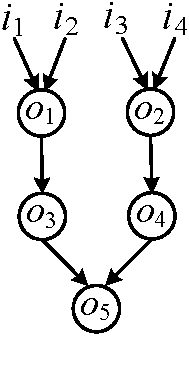
\includegraphics[width=0.16\linewidth]{Visio/sequencing_graph.pdf}}
    \label{ta}
	\subfloat[]{
        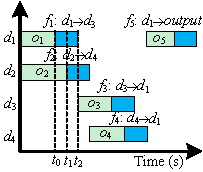
\includegraphics[width=0.42\linewidth]{Visio/scheduling.pdf}}
    \label{tb}
    \subfloat[]{
        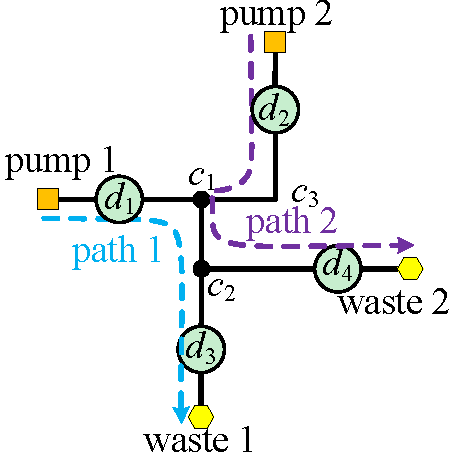
\includegraphics[width=0.35\linewidth]{Visio/chip_architecture.pdf}}
    \label{tc}
	  \caption{Flow-path planning. (a) Sequencing graph of a bioassay. (b) A scheduling and binding solution with minimized execution time. (c) Flow paths constructed on a given chip architecture.}
	  \label{fig:motivation}
%\vspace{-0.5cm}
\end{figure}

\subsection{Design Challenges in Flow-Path Planning}\label{sec:flow_path_chan}

When executing bioassays on a microfluidic biochip, fluid samples need to be transported to specific devices/channel segments at certain time windows according to the scheduling and binding solution and this, undoubtedly, requires a carefully planned flow-channel network to complete these tasks. For a  transportation task between two devices denoted as $d_i$ and $d_j$, to drive the movement of fluid, an external pressure source or a mechanical pump needs to be connected to $d_i$ to produce thrust. Moreover, to avoid channel blockage after the completion of the corresponding operation, waste liquid that is not needed anymore should be discarded, thus requiring a waste port connected to $d_j$. As a consequence, the pump, the two devices, the waste port, as well as the channel segments connecting them form the complete flow path of the transportation task.

We take the sequencing graph shown in Fig.~\ref{fig:motivation}(a) as an example to illustrate the flow-path planning on a certain biochip. Fig.~\ref{fig:motivation}(b) shows a scheduling and binding solution with minimized execution time of the bioassay described in Fig.~\ref{fig:motivation}(a), where four devices ($d_1$--$d_4$) are allocated and five transportation tasks ($f_1$--$f_5$) are scheduled to execute corresponding operations. For example, in task $f_1$, the resulting fluid of operation $o_1$ is required to be transported to device $d_3$ as an input sample of operation $o_3$, leading to a flow path from $d_1$ to $d_3$. Fig.~\ref{fig:motivation}(c) shows a given biochip architecture, on which $path\;1$ is a feasible flow path starting with a mechanical pump, passing through devices $d_1$ and $d_3$, and ending at a waste port. Note that a valid flow path should bypass those devices  occupied by other on-going operations as well as flow channels used for fluid caching.

\begin{figure*}[t]
    \centering
	 \subfloat[]{
       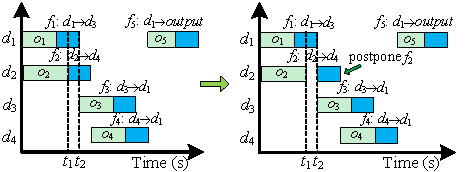
\includegraphics[width=0.55\linewidth]{Visio/scheduling_adjustment.pdf}}
    \label{ta1}
	\subfloat[]{
        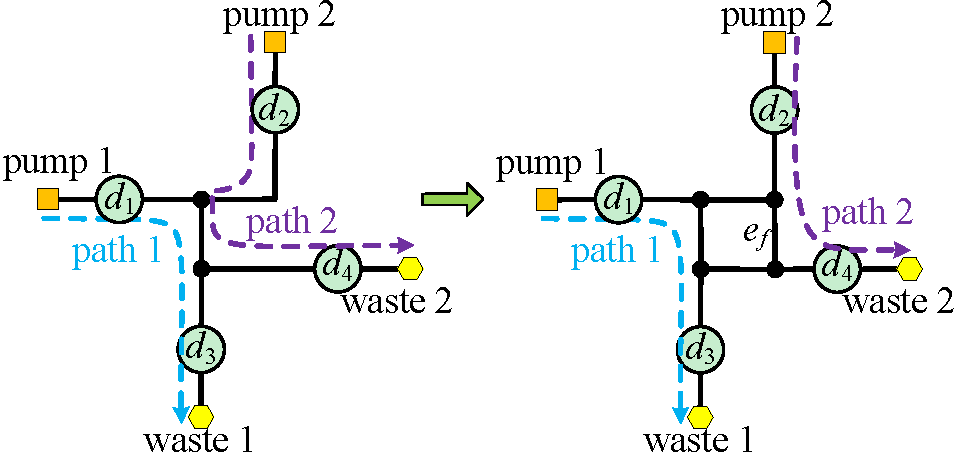
\includegraphics[width=0.43\linewidth]{Visio/new_path.pdf}}
    \label{tb1}
	  \caption{Strategies for transportation conflict elimination. (a) Scheduling adjustment. (b) Architecture ajustment.}
	  \label{fig:strategy}
%\vspace{-0.5cm}
\end{figure*}

\subsubsection{Transportation conflict}

Since several transportation tasks may be performed concurrently in a scheduling scheme,
to avoid potential transportation conflicts, flow paths among these tasks need to be considered systematically. Let us revisit the scheduling scheme in Fig.~\ref{fig:motivation}(b). Since the time windows for executing transportation tasks $f_1$ and $f_2$ overlap with each other, the corresponding flow paths cannot share any on-chip resource, including pump ports, channel segments, etc. For example, $path\;1$ and $path\;2$ in Fig.~\ref{fig:motivation}(c) are flow paths constructed for tasks $f_1$ and $f_2$, respectively. These two paths, however, are essentially in transportation conflict with each other, since switches $c_1$ and $c_2$ as well as the channel segment between them are shared by both paths. Worse still, we cannot even find a valid path-planning solution for the two tasks due to the limited on-chip resources in Fig.~\ref{fig:motivation}(c).

Accordingly, we propose two conflict elimination techniques, \textsl{scheduling adjustment} and \textsl{architecture adjustment} as illustrated in Fig.~\ref{fig:strategy}, to fundamentally solve the transportation conflict discussed above. %Note that when two fluidic flows pass through the same channel segment one after the other, the second flow can be contaminated by the residue left behind by the first flow, resulting in a cross-contamination between them. This problem can be solved by injecting a buffer fluid into the chip to wash the corresponding channels \cite{hu2015wash}.


\begin{easylist}
&\textit{Scheduling adjustment}: The goal of scheduling adjustment is to eliminate transportation conflicts in a flow-path planning solution by postponing the execution of some transportation tasks. As illustrated in Fig.~\ref{fig:strategy}(a), to eliminate the conflict between the flow paths described in Fig.~\ref{fig:motivation}(c), the execution of transportation task $f_2$ is postponed by the scheduling adjustment operation, so that tasks $f_1$ and $f_2$ do not overlap in their execution time. As a result, the shared channel segment between switches $c_1$ and $c_2$ in Fig.~\ref{fig:motivation}(c) can be used by both paths sequentially, although the completion time of the bioassay is increased slightly.
%Although the execution of the complete bioassay might be postponed by the scheduling adjustment, a slight increase of completion time is acceptable, for the benefit of the complete elimination of transportation conflicts.

&\textit{Architecture adjustment}: Another strategy to eliminate the transportation conflicts is to introduce extra resources to the biochip architecture directly, so that the previously shared on-chip resources can be released from conflicts. For example, in Fig.~\ref{fig:strategy}(b), a channel segment $e_f$ with two extra switches is added to the chip architecture, leading to a new flow path for transportation task $f_2$. Since the new path does not share any resource with that of task $f_1$, the previous conflict is removed from the chip successfully.

\end{easylist}

\subsubsection{Caching deadlock}

\begin{figure}[t]
    \centering
	 \subfloat[]{
       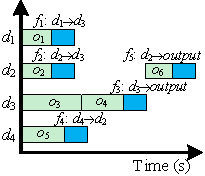
\includegraphics[width=0.5\linewidth]{Visio/caching_deadlock1.pdf}}
    \label{ta}
	\subfloat[]{
        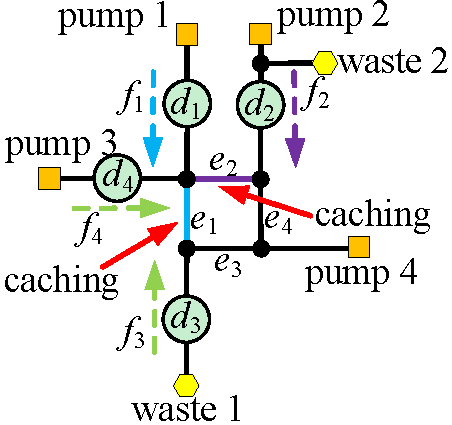
\includegraphics[width=0.44\linewidth]{Visio/caching_deadlock2.pdf}}
    \label{tb}
	  \caption{Illustration of caching deadlock. (a) Scheduling scheme of a bioassay. (b) A flow-path planning solution with caching deadlock.}
	  \label{fig:deadlock}
%\vspace{-0.5cm}
\end{figure}

Another issue that needs to be considered during flow-path planning is caching deadlock. Since flow channels in a distributed channel-storage architecture fulfill the dual functions of transportation and caching, channel segments used for fluid caching may block the normal transportation of other fluids, thereby leading a deadlock of the flow-channel network. For example, when mapping the scheduling scheme described in Fig.~\ref{fig:deadlock}(a) to the biochip architecture shown in Fig.~\ref{fig:deadlock}(b), the resulting fluids of operations $o_1$ and $o_2$ need to be transported from devices $d_1$ and $d_2$ to $d_3$, respectively. To wait for the completion of operation $o_3$, whose resulting fluid is another input of operation $o_4$, the two fluids are temporally cached in channel segments $e_1$ and $e_2$, and thus blocking the flow path of transportation task $f_4$. To solve this problem, one feasible solution is to desynchronize the execution of these transportation tasks by employing an idea similar to the proposed scheduling adjustment strategy. For example, if the execution of $f_4$ is postponed to a point in time that the fluid cached in either $e_1$ or $e_2$ has been removed, the deadlock in Fig.~\ref{fig:deadlock}(b) can be eliminated. Another way to solve this problem is to release these blocked channels by directly moving the corresponding cached fluids to other unused channel segments. For example, if the resulting fluid of $o_2$ is moved to either channel segment $e_3$ or $e_4$ for caching, the deadlock can also be eliminated.

\subsection{Problem Formulation}

Based on the proposed concept of distributed channel storage, the synthesis problem considering architecture design and path planning in flow-based microfluidic biochips can be formulated as follows:

\begin{easylist}
&\textit{Inputs}: The sequencing graph of a biochemical assay;
the execution duration of all operations; the maximum numbers of devices allowed
in the chip.

&\textit{Outputs}: A schedule minimizing intermediate fluid storage; a channel
caching schedule including the locations and the time slots
of fluid samples stored temporarily in channels; a biochip architecture with the exact flow paths to manipulate the transportation/caching of fluid samples without conflict.

&\textit{Objectives}: Minimizing the overall resource usage and the completion time of the bioassay.
\end{easylist}



15 gid=3000000
15 uid=3603518
25 ctime=1538382170.5264
27 atime=1538916861.459084

\section{Synthesis of Biochips Considering Storage and Caching}
\label{sec:storage_synthesis}

Storage and caching should be considered from scheduling to architectural synthesis
to reduce storage requirements and to construct channels for distributed
storage.
Correspondingly, the proposed method includes three major parts:
1) intermediate fluid storage is minimized in scheduling and binding,
2) all the allocated devices are assigned to exact locations on a biochip, and 3) channel segments that cache intermediate fluid samples are constructed among devices, leading to a
distributed channel-storage system which fulfills the tasks of transportation and storage at the same time.

\subsection{Minimizing Storage in Scheduling and Binding}
\label{sec:scheduling_binding}

Scheduling and binding assign operations in a given sequencing graph
to time slots of specific devices.
To optimize storage requirements,
we formulate the scheduling and binding task as
an ILP problem. %instead of the commonly used List algorithm.

The variables and constraints for scheduling and binding are listed in
Table~\ref{tb:vc_scheduling_binding}. The uniqueness constraint (\ref{eq:uniqueness})
specifies that operation $o_i$ should be assigned
to one device only. The duration constraint ensures
$o_i$ has enough time to finish.
The precedence constraint (\ref{eq:precedence}) guarantees that a child
operation must be executed later than its parents. Finally, the
non-overlapping constraint (\ref{eq:non_overlapping}) prevents two operations
whose operation periods overlap from being executed by the same device.
These constraints are common for high-level synthesis and
widely used in synthesis methods for biochips \cite{SuCh04}.

To minimize the execution time of the assay, another variable $t^E$ is
used to represent
the latest ending time of all operations, constrained as
\begin{equation}\label{eq:latest_finishing}
t^e_i \le t^E,  \quad \forall o_i\in O.
\end{equation}
\vskip 7pt
By minimizing $t^E$, the operations in the sequencing graph
are assigned to proper time slots %as early as possible
to produce a compact schedule.



To reduce storage requirements, we introduce an additional \textit{storage minimization
objective}.
\textcolor{red}{Assume that the pure transportation time from a device to another device
is a constant $u_c$.}
If the schedule produces a transportation time larger
than $u_c$, the fluid sample must be cached somewhere before it is
used ($u_c$ is set to 1 in our experiments).
Fig.~\ref{fig:schedule_storage} illustrates
the schedules of executing an assay with five operations by two devices. The sequencing graph of this assay is shown in Fig.~\ref{fig:schedule_storage}(a).
In \figname~\ref{fig:schedule_storage}(b),
operation $o_2$ is scheduled before $o_3$. Consequently, the result of $o_2$
must be stored until it is used by $o_4$ and $o_5$, leading to two storage
requirements. %lasting six time units in total.
In \figname~\ref{fig:schedule_storage}(c), $o_3$ is scheduled before $o_2$,
leading to only one storage requirement lasting a shorter time.
In this example, we can observe that
the lifetime of stored fluid samples is determined by the difference between
the ending time of the parent operation and the starting time of the child
operation $u_{i,j}$ defined in Table~\ref{tb:vc_scheduling_binding}. Consequently, the total storage requirement can be reduced by
solving the following ILP problem:
\begin{align}
\text{minimize} & \quad \alpha t^E+\beta\sum_{{(o_i,o_j)\in E\bigwedge d_i\ne d_j }}u_{i,j}
 \label{eq:minobj}\\
\text{subject to} & \quad
\text{(\ref{eq:uniqueness})--(\ref{eq:latest_finishing}})\label{eq:op_cond}
\end{align}
where $\alpha$ and $\beta$ are constants to control the priority of
execution time and storage requirement minimization.
$d_i \ne d_j $ excludes the operation pairs assigned to the same device
so that they do not need transportation.


\begin{figure}[t]
{\figurefontsize
\centering
\input{Fig/schedule_storage.pdf_tex}
\caption{Storage reduction. (a) Sequencing graph. (b) Schedule with two
storage requirements. (c) Schedule with one storage requirement. The execution
times of the assay with these two schedules are equal. }
\label{fig:schedule_storage}
}
%\vspace{-0.5cm}
\end{figure}



\subsection{Architectural Synthesis with Distributed Channel Storage}\label{sec:channel_storage_synthesis}
After solving the
optimization problem (\ref{eq:minobj})--(\ref{eq:op_cond}), we have a schedule
similar to \figname~\ref{fig:schedule_storage}(c),
including the information: 1) to which devices operations are
assigned; 2) the starting time and the ending time of each operation; 3) the
starting time and the ending time of each fluid storage requirement.

The schedule, however, only defines the transportation requirements between
devices after operations are executed. In the chip, physical channels need
be constructed to conduct these transportation tasks.
When a large assay is executed by several devices,
transportation channels need to be built between nearly
any pair of devices to move fluid samples
efficiently.
Since the flow-layer in a biochip is only two-dimensional, eventually
intersections between channels cannot be avoided. At an intersection,
a switch should be built to direct the transportation
flow to the target device. A switch is constructed by
four valves at an intersection, as shown in \figname~\ref{fig:switch}(a). At a
given moment, two out of the four valves in a switch are opened to
connect two channel segments. Consequently, a transportation
channel between two devices becomes a path
formed by several channel segments connected by switches.
Such a path is called a \textit{transportation path} henceforth.

Besides channels, the locations of devices should also be determined.
These locations should be assigned together with the construction of
transportation channels, because the distance and relative locations of devices
affect how channels are constructed and how they intersect with each other.

Considering devices and channels together, the architecture of a biochip can
be described as devices surrounded by channel segments in the form of a grid.
For example, the architecture of a biochip with five devices is
shown in \figname~\ref{fig:switch}(b), where the smaller nodes
represent switches and the larger nodes represent devices.
Transportation paths between devices are
formed from channel segments connected by switches, e.g., path 1 and path 2
in \figname~\ref{fig:switch}(b).
Since transportation paths are used only when there is a fluid sample
traveling along it, channel segments can be reused by
different paths so that the efficiency of channel segments increases.


\begin{figure}[t]
{\figurefontsize
\centering
\input{Fig/switch.pdf_tex}
\caption{Switch and channel storage. Large nodes represent devices and
small nodes represent switches.  (a) Switch structure. (b) Two paths
sharing one channel segment with time multiplexing. (c) Fluid sample to
channel storage. (d) Storage in channel segment. (d) Fluid sample from channel
storage to device.}
\label{fig:switch}
}
%\vspace{-0.5cm}
\end{figure}

With transportation paths formed from channel segments, the proposed
distributed channel storage concept can thus be formulated.
As illustrated in \figname~\ref{fig:device_storage}(c),
a dedicated storage unit suffers bandwidth problem at its ports
because multiple fluid samples must be queued when they access the storage unit
at the same time.
Observing that the storage cells
inside a dedicated storage unit
are in fact channel segments, as shown in
\figname~\ref{fig:valve_mixer_storage}(c), we distribute fluid storage
directly in channel segments. For example, in
\figname~\ref{fig:switch}(c), along path 3 a fluid sample is moved to the channel
segment between A and B. However, the next operation using this
fluid sample is scheduled later, so that the fluid sample must stay in the
channel segment. During the lifetime of this storage, the channel segment
between A and B cannot
be used by other paths
and the valves at the two ends of this channel segment should be closed.
Further transportation tasks between devices are, however, still
fulfilled by paths not including this channel segment,
as path 4 and 5 in \figname~\ref{fig:switch}(d).
When the stored fluid sample is finally needed, it is moved to the target
device again by a newly constructed transportation path, shown as path 6
in \figname~\ref{fig:switch}(e).

Unlike the dedicated storage unit shown in
\figname~\ref{fig:valve_mixer_storage}(c), the distributed storage in a
channel segment has a higher access efficiency.
When a fluid sample stays in a channel segment,
that segment is turned into a \textit{storage segment}. When the
fluid sample moves again, the segment becomes a part of
the transportation path. This concept of channel role switching
unifies transportation and storage,
and
the low-efficiency channels forming storage cells
in a dedicated storage unit are excluded completely.
In addition, this on-the-spot caching is closer to the target
device than a dedicated storage unit, so that the execution efficiency of
the assay can also be improved.

\begin{figure}[t]
{\figurefontsize
\centering
\input{Fig/grid_model.pdf_tex}
\caption{Connection grid.}
\label{fig:grid_model}
}
%\vspace{-0.5cm}
\end{figure}

To synthesize the architecture of a biochip from its schedule requires to
determine the relative locations of devices
as well as channel segments and the switches connecting them as shown by the examples
in  \figname~\ref{fig:switch}(b)--(e). The devices, switches and their connections together form a
\textit{connection graph}. %nodes edges}
A valid connection graph should be capable of
constructing all transportation paths specified in the schedule and caching
intermediate fluid samples in channel segments.
To reduce resource usage, the synthesized connection graph
should contain as few edges as possible.

The connection graph is generated using a general \textit{connection grid}, as
shown in \figname~\ref{fig:grid_model}. At each node $n_i$ on the grid,
either a device or a switch can be assigned. An edge $e_j$ represents
a channel segment capable of caching a fluid sample.
We use a 0-1 variable $a_{i,k}$ to represent whether device $d_k$
is assigned to node $n_i$. Since a node can be occupied by no more than one device
and a device must be assigned once, $a_{i,k}$ can be constrained as
\begin{equation} \label{eq:device_node_1}
\sum_{d_k\in D} a_{i,k}\le 1, \forall n_i\in N, \quad
\sum_{n_i\in N} a_{i,k}=1, \forall d_k\in D
\end{equation}
where $N$ is the set of nodes in the connection grid and $D$ is the set of
devices.

Assume there is a transportation path $p_r$ between
device $d_{k_1}$ and device $d_{k_2}$ in the period between
$t^s_{r}$ and ${t^e_{r}}$, where $r$ is the index of the path.
$t^s_{r}$ and ${t^e_{r}}$ are constants determined in the
scheduling and binding step in Section~\ref{sec:scheduling_binding}.
We use a 0-1 variable $\epsilon_{j,r}$ to represent whether the edge
$e_j$ is on the path $p_r$.
To construct a path between $d_{k_1}$ and $d_{k_2}$, we need to
guarantee that the path starts from the node for $d_{k_1}$
and ends at the node for $d_{k_2}$.
Consequently, at one of these two nodes, only one of the four edges incident
to the node can be covered in the path.
At each other node on the path, exactly two edges are covered by the path, as
illustrated with path $p_r$ in \figname~\ref{fig:grid_model}.
Accordingly, we can
construct the path with the following constraints
\begin{equation}\label{eq:degree}
\sum_{e_j\in E_i}{\epsilon_{j,r}}\ge 2-a_{i, k_1}-a_{i, k_2}-(1-y_{i,r})M,
\sum_{e_j\in E_i}{\epsilon_{j,r}}\le y_{i,r}M
\end{equation}
where $E_i$ is the set of edges incident to node $n_i$; $y_{i,r}$ is an
auxiliary 0-1 variable to indicate
whether there is an edge on $p_r$ that is incident to $n_i$;
$M$ is a very large constant to transform the two
situations indicated by $y_{i,r}$ into linear constraints
\cite{chen2011applied}.
The path construction constraints become more complex when a storage is involved,
            which leads to three sub-paths: 1) from $d_{k_1}$ to a storage segment; 2)
            the storage segment caching the fluid sample; 3) from the storage segment to the
            target device $d_{k_2}$.
            We denote the three transportation paths as $p_{r, 1}$,
            $p_{r, 2}$ and $p_{r,3}$, as illustrated in \figname~\ref{fig:grid_model}.
            Since the end node of $p_{r,1}$ and the starting
            node of $p_{r, 3}$ can be any node on the connection grid as long as they are
            the two end nodes of the same edge,
            we use 0-1 variable $a_{i_1,r_1}$ to represent that node
            $n_{i_1}$ is the last node on the path $p_{r,1}$ and the
            variable $a_{i_2,r_2}$ to represent that node
            $n_{i_2}$ is the first node on the path $p_{r,2}$.
            Afterwards, we create constraints similar to (\ref{eq:degree}) for each
            sub path. In addition, we include the constraint that $n_{i_1}$ and $n_{i_2}$
            are the two end nodes of the same edge.

In the schedule, there are many transportation paths
at a given moment. These paths should not
intersect at a node or share the same edge to avoid conflict.
Therefore, we examine the paths on the connection grid at the starting time of each
transportation path, because this is the moment a new transportation is
initiated. At each such moment $t$, we constrain that all the paths existing on
the connection grid should not share any edge or intersect at a node, as,
\begin{equation}\label{eq:edge_node_sharing}
\sum_{e_j\in E} \epsilon_{j,r}\le 1, \forall p_r\in P_t, \quad
\sum_{n_i\in N} \eta_{i,r}\le 1, \forall  p_r\in P_t
\end{equation}
where $P_t$ is the set of paths existing at time $t$;
$\eta_{i,r}$ represents whether node $n_i$ is on path $p_r$;
$E$ and $N$ are the sets
of edges and nodes in the connection grid, respectively. Exception of
constraint (\ref{eq:edge_node_sharing}) is that the two ending nodes of the
storage segment $p_{r,2}$ can be passed by other paths when the fluid sample is stored,
as path $p'_r$ in \figname~\ref{fig:grid_model}, so that their variables
$\eta_{i,r}$ are not included in (\ref{eq:edge_node_sharing}) when $p_{r,2}$
exists. %in the grid.

When generating the architecture of the chip, we minimize the number of edges
that are really used by the transportation paths
to reduce resource usage. If an edge is used once by any transportation path,
it should appear in the chip. We use a 0-1 variable $s_j$ to represent whether
a channel segment should be kept in the chip, and constrain it as
\begin{equation}\label {eq:edge_app}
s_j\ge \epsilon_{i,r}, \; \forall p_r\in P
\end{equation}
where $P$ is the set including all transportation paths.

Finally, the architecture of the biochip can be determined by solving the
following optimization problem
\begin{align} \label{eq:edge_opt}
\text{minimize} & \quad \sum_{e_j\in E}s_j\\
\text{subject to} & \quad
\text{(\ref{eq:device_node_1})--(\ref{eq:edge_app})}\label{eq:edge_opt_cond}
\end{align}
After determining $s_j$, the edges and nodes
that are not used in the connection grid
are removed to generate the chip architecture as a planar
connection graph similar to
\figname~\ref{fig:switch}(b)--(e).




\subsection{\textcolor{red}{Scheduling Recomputation}}\label{sec:schedual_recomputation}
\textcolor{red}{
As discussed previously, since the layout of the biochip has not been determined during the high-level synthesis stage, we use a constant $u_c$ to estimate the durations of transportation tasks. After completing the architectural synthesis above, a biochip architecture that defines the  positions of devices and the corresponding connections among them is generated. With this chip architecture, the execution time of each transportation task in the scheduling can be computed directly. Thereafter, the generated chip architecture is fed back into the high-level synthesis stage by re-performing the proposed scheduling method, thus updating the execution procedure of the complete bioassay with accurate transportation latencies. Note that the velocity of fluid flow is set to 10 mm/s in the our method \cite{minhass2012architectural}.
}











15 gid=3000000
15 uid=3603518
27 mtime=1539613900.189551
26 ctime=1539613900.19055
27 atime=1539613900.230547

%%% this file is called up by thesis.tex
% content in this file will be fed into the main document

\chapter{Discussion} % top level followed by section, subsection


% ----------------------- paths to graphics ------------------------

% change according to folder and file names
\ifpdf
    \graphicspath{{7/figures/PNG/}{7/figures/PDF/}{7/figures/}}
\else
    \graphicspath{{7/figures/EPS/}{7/figures/}}
\fi


% ----------------------- contents from here ------------------------






% ---------------------------------------------------------------------------
% ----------------------- end of thesis sub-document ------------------------
% ---------------------------------------------------------------------------
\section{Simulation Results}\label{sec:results}

The proposed framework was implemented in C++ and tested
using a \SI[mode=text]{3.20}{\GHz} CPU with 
\SI{8}{GB} memory.
We demonstrate
the results using FPVAs with valves in different rows and columns. The
tested arrays are shown in Table I, where the first column shows
the dimensions of the arrays and the second column shows
the number of valves. 
We used Gurobi \cite{gurobi} to solve the optimization problems in the
proposed method.

The results of testing FPVAs with a single pressure source and a single pressure sensor
are shown in Table~\ref{tb_test}.
% These arrays contain long channels for transportation and obstacle areas without
% valves. 
%The numbers of valves in the arrays are shown in the column $n_v$.  
%These numbers are calculated by multiplying
%the row number and column number and subtracting
%the number of valves not built due to channels and obstacles.
The direct approach is the method published in \cite{CBBK17}, which
does not use loop relaxation introduced in Section~\ref{sec:loop_relax} for
acceleration. In Table~\ref{tb_test}, the
numbers of test paths are shown in the column $n^d_p$. The CPU time to
generate these patterns is shown in the column $t^d_p$. The columns $n^d_c$ and
$t^d_c$ show the number of cut patterns and the CPU time to generate them.
The columns $n^d_l$ and $t_l^d$ show the number of patterns for testing leakage in the
control layer and the CPU time to generate these patterns. The
total number of test patterns is shown in the column $N^d$. 
``*'' means that no valid results are available 
%from the corresponding approach 
due to runtime.
According to these results, the direct approach suffers from the scalability problem
due to its pure ILP formulation.
%Though the flow path test patterns can still be found with the valve array of
%the size $20\times20$, the cut patterns cannot be generated.
In these results, the number of cuts is much larger than the number of test
paths. This is because a path can travel through many valves in a zigzag shape and 
only a few orthogonal paths can already cover all the valves.
However, the cuts required to cover all the valves in an
FPVA is proportional to the size of the array, leading a much larger number of
such test patterns.

\begin{figure}[t]
{\figurefontsize
\centering
\pgfplotsset{compat=1.3,
    %legend drawing style, single bar instead of the default double mini bars
    /pgfplots/ybar legend/.append style={ 
        /pgfplots/legend image code/.code={%
           \draw[##1,/tikz/.cd,yshift=-0.25em]
           (0cm,0cm) rectangle (5pt,0.8em);
        },
    }
}
\begin{tikzpicture}
\begin{axis}[
% x=1.1cm, y=0.25cm, ymax=12, line width=0.75pt,
x=1.1cm, y=1.40, ymax=55, line width=0.75pt,
xlabel={FPVAs with different size}, xlabel shift=-5pt,
ylabel={Number of test patterns}, ylabel shift=0pt, 
xtick={1,...,6},xticklabels={$5\times5$, $10\times10$, $15\times15$, $20\times20$, $25\times25$, $30\times30$},
x tick label style={rotate=330, xshift=-15pt,yshift=-8pt,anchor=west}, 
xticklabel pos=left, xtick align=outside, xtick pos=left,
ytickmin=0,ytickmax=40,
% ymin = 0,
% ymax = 1,
ytick={0,10,20,30}, yticklabels={0,10,20,30},
legend columns=4, legend style={at={(0.5,0.88)}, anchor=center, nodes={inner xsep=0pt},
draw=none, column sep=5pt},
ybar=0pt, bar width=7
]

   \addplot[line width=0.5pt, black, fill=orange!70!white] table[x=size,y=2port] 
{port_testvector_number.dat};
   \addplot[line width=0.5pt, black, fill=blue!65!orange] table[x=size,y=3port] 
{port_testvector_number.dat};
   \addplot[line width=0.5pt, black, fill=blue!40!orange] table[x=size,y=4port] 
{port_testvector_number.dat};
   \addplot[line width=0.5pt, black, fill=blue!80!orange] table[x=size,y=5port] 
{port_testvector_number.dat};
   \legend{3 Ports\hspace*{0.5pt}, 4 Ports\hspace*{0.5pt}, 5 Ports\hspace*{0.5pt}, 6 Ports\hspace*{0.5pt}}
\end{axis}
\end{tikzpicture}

%\begin{tikzpicture}
\begin{axis}[
% x=1.1cm, y=0.25cm, ymax=12, line width=0.75pt,
x=1.1cm, y=1.40, ymax=60, line width=0.75pt,
ylabel={Cut-set Test Vector Number}, ylabel shift=-6pt, 
xtick={1,...,6},xticklabels={$5\times5$, $10\times10$, $15\times15$, $20\times20$, $25\times25$, $30\times30$},
x tick label style={rotate=330, xshift=-15pt,yshift=-5pt,anchor=west}, 
xticklabel pos=left, xtick align=outside, xtick pos=left,
ytickmin=0,ytickmax=40,
% ymin = 0,
% ymax = 1,
ytick={0,5,10,15,20,25,30,35,40}, yticklabels={0,5,10,15,20,25,30,35,40},
legend columns=4, legend style={at={(0.5,0.9)}, anchor=center, nodes={inner xsep=2pt},
draw=none, column sep=1pt},
ybar=0pt, bar width=7
]

   \addplot[line width=0.5pt, black, fill=orange!70!white] table[x=size,y=2port] 
{port_cut_number.dat};
   \addplot[line width=0.5pt, black, fill=blue!65!orange] table[x=size,y=3port] 
{port_cut_number.dat};
   \addplot[line width=0.5pt, black, fill=blue!40!orange] table[x=size,y=4port] 
{port_cut_number.dat};
   \addplot[line width=0.5pt, black, fill=blue!80!orange] table[x=size,y=5port] 
{port_cut_number.dat};
   \legend{3 Ports\hspace*{0.5pt}, 4 Ports\hspace*{0.5pt}, 5 Ports\hspace*{0.5pt}, 6 Ports\hspace*{0.5pt}}
\end{axis}
\end{tikzpicture}
%%\begin{tikzpicture}
\begin{axis}[
x=1.1cm, y=0.26cm, ymax=12, line width=0.75pt,
ylabel={Exec./Valve Ratio}, ylabel shift=-6pt, 
xtick={1,...,6},xticklabels={RA100, RA70, CPA, RA30, IVD, PCR},
x tick label style={rotate=330, xshift=-15pt,yshift=-5pt,anchor=west}, 
xticklabel pos=left, xtick align=outside, xtick pos=left,
ytickmin=0,ytickmax=10, 
ytick={0,5,10}, yticklabels={0,0.5,1},
legend columns=2, legend style={at={(0.5,0.9)}, anchor=center, nodes={inner xsep=2pt},
draw=none, column sep=1pt},
ybar=0pt, bar width=7
]
   \addplot[line width=0.5pt, black, fill=orange!70!white]
table[x=cir,y=exetime] 
{exe_time_valve_cmp.dat};
   \addplot[line width=0.5pt, black, fill=blue!65!orange] table[x=cir,y=valve] 
{exe_time_valve_cmp.dat};
   \legend{Execution Time\hspace*{9pt}, Valve\hspace*{8pt}}
\end{axis}
\end{tikzpicture}

\caption{Comparison of numbers of test patterns for FPVAs with different
numbers of ports.}
\label{fig:port_test}
}
\end{figure}

\begin{figure}[t]
{\figurefontsize
\centering
\pgfplotsset{compat=1.3,
    %legend drawing style, single bar instead of the default double mini bars
    /pgfplots/ybar legend/.append style={ 
        /pgfplots/legend image code/.code={%
           \draw[##1,/tikz/.cd,yshift=-0.25em]
           (0cm,0cm) rectangle (5pt,0.8em);
        },
    }
}
\begin{tikzpicture}
\begin{axis}[
% x=1.1cm, y=0.25cm, ymax=14, line width=0.75pt,
x=1.1cm, y=9.00, ymax=9, line width=0.75pt,
xlabel={FPVAs with different size},xlabel shift=-5pt,
ylabel={Number of test trees}, ylabel shift=0pt, 
xtick={1,...,6},xticklabels={$5\times5$, $10\times10$, $15\times15$, $20\times20$, $25\times25$, $30\times30$},
x tick label style={rotate=330, xshift=-15pt,yshift=-8pt,anchor=west}, 
xticklabel pos=left, xtick align=outside, xtick pos=left,
ytickmin=0,ytickmax=6,
% ymin = 0,
% ymax = 1,
ytick={2,4,6}, yticklabels={2,4,6},
legend columns=4, legend style={at={(0.5,0.86)}, anchor=center, nodes={inner xsep=0pt},
draw=none, column sep=5pt},
ybar=0pt, bar width=7
]

   \addplot[line width=0.5pt, black, fill=orange!70!white] table[x=size,y=5] 
{hole_wall_path.dat};
   \addplot[line width=0.5pt, black, fill=blue!65!orange] table[x=size,y=10] 
{hole_wall_path.dat};
   \addplot[line width=0.5pt, black, fill=blue!40!orange] table[x=size,y=15] 
{hole_wall_path.dat};
   \addplot[line width=0.5pt, black, fill=blue!80!orange] table[x=size,y=20] 
{hole_wall_path.dat};
   \legend{5\% \hspace*{0.5pt}, 10\% \hspace*{0.5pt},15\%\hspace*{0.5pt},20\%\hspace*{0.5pt}}
\end{axis}
\end{tikzpicture}
\vskip 10pt\pgfplotsset{compat=1.3,
    %legend drawing style, single bar instead of the default double mini bars
    /pgfplots/ybar legend/.append style={ 
        /pgfplots/legend image code/.code={%
           \draw[##1,/tikz/.cd,yshift=-0.25em]
           (0cm,0cm) rectangle (5pt,0.8em);
        },
    }
}
\begin{tikzpicture}
\begin{axis}[
% x=1.1cm, y=0.25cm, ymax=14, line width=0.75pt,
x=1.1cm, y=1.40, ymin=0, ymax=49.5, line width=0.75pt,
xlabel={FPVAs with different size}, xlabel shift=-5pt,
ylabel={Number of cuts}, ylabel shift=0pt, 
xtick={1,...,6},xticklabels={$5\times5$, $10\times10$, $15\times15$, $20\times20$, $25\times25$, $30\times30$},
x tick label style={rotate=330, xshift=-15pt,yshift=-8pt,anchor=west}, 
xticklabel pos=left, xtick align=outside, xtick pos=left,
ytickmin=0,ytickmax=40,
% ymin = 0,
% ymax = 1,
ytick={10,20,30}, yticklabels={10,20,30},
legend columns=4, legend style={at={(0.5,0.86)}, anchor=center, nodes={inner xsep=0pt},
draw=none, column sep=5pt},
ybar=0pt, bar width=7
]

   \addplot[line width=0.5pt, black, fill=orange!70!white] table[x=size,y=5] 
{hole_wall_cut.dat};
   \addplot[line width=0.5pt, black, fill=blue!65!orange] table[x=size,y=10] 
{hole_wall_cut.dat};
   \addplot[line width=0.5pt, black, fill=blue!40!orange] table[x=size,y=15] 
{hole_wall_cut.dat};
   \addplot[line width=0.5pt, black, fill=blue!80!orange] table[x=size,y=20] 
{hole_wall_cut.dat};
   \legend{5\% \hspace*{0.5pt}, 10\% \hspace*{0.5pt},15\%\hspace*{0.5pt},20\%\hspace*{0.5pt}}
\end{axis}
\end{tikzpicture}

%\begin{tikzpicture}
\begin{axis}[
x=1.1cm, y=0.26cm, ymax=12, line width=0.75pt,
ylabel={Exec./Valve Ratio}, ylabel shift=-6pt, 
xtick={1,...,6},xticklabels={RA100, RA70, CPA, RA30, IVD, PCR},
x tick label style={rotate=330, xshift=-15pt,yshift=-5pt,anchor=west}, 
xticklabel pos=left, xtick align=outside, xtick pos=left,
ytickmin=0,ytickmax=10, 
ytick={0,5,10}, yticklabels={0,0.5,1},
legend columns=2, legend style={at={(0.5,0.9)}, anchor=center, nodes={inner xsep=2pt},
draw=none, column sep=1pt},
ybar=0pt, bar width=7
]
   \addplot[line width=0.5pt, black, fill=orange!70!white]
table[x=cir,y=exetime] 
{exe_time_valve_cmp.dat};
   \addplot[line width=0.5pt, black, fill=blue!65!orange] table[x=cir,y=valve] 
{exe_time_valve_cmp.dat};
   \legend{Execution Time\hspace*{9pt}, Valve\hspace*{8pt}}
\end{axis}
\end{tikzpicture}

\caption{Comparison of numbers of test patterns for 
FPVAs with different numbers of long channels and obstacles.}
\label{fig:wall_hole_test}
}
\end{figure}

\begin{table*}[t] 
\centering
{\footnotesize
\renewcommand{\tabcolsep}{10.35pt}
\renewcommand{\arraystretch}{1}
\caption{Comparison between test patterns generated by the proposed method
and the ATPG-based method}
\label{tb_tradition}
\begin{tabular}{ c  c  c c c c c} \hlinewd{0.7pt}
\multicolumn{3}{c}{Proposed method} &
\multicolumn{1}{c}{} &
\multicolumn{3}{c}{ATPG-based method \cite{HuYHC14}}\\
% \multicolumn{1}{c}{} &
% \multicolumn{7}{c}{Acceleration} \\
\cline {1-3}\cline {5-7}
\multicolumn{1}{c}{} &
\multicolumn{1}{c}{Test Pattern} &
\multicolumn{1}{c}{Detected Faults} &
\multicolumn{1}{c}{} &
\multicolumn{1}{c}{} &
\multicolumn{1}{c}{Test Pattern} &
\multicolumn{1}{c}{Detected Faults}\\
% \multicolumn{1}{c}{$n^d_p$} &
% \multicolumn{1}{c}{$t^d_p(s)$} &
% \multicolumn{1}{c}{$n^d_c$} &
% \multicolumn{1}{c}{$t^d_c(s)$} &
% \multicolumn{1}{c}{$n^d_l$} &
% \multicolumn{1}{c}{$t^d_l(s)$} &
% \multicolumn{1}{c}{$N^d$} &
% % \multicolumn{1}{c}{$T^d(s)$} &
% \multicolumn{1}{c}{} &
% \multicolumn{1}{c}{$n^a_p$} &
% \multicolumn{1}{c}{$t^a_p(s)$} &
% \multicolumn{1}{c}{$n^a_c$} &
% \multicolumn{1}{c}{$t^a_c(s)$} &
% \multicolumn{1}{c}{$n^a_l$} &
% \multicolumn{1}{c}{$t^a_l(s)$} &
% \multicolumn{1}{c}{$N^a$} \\
% \multicolumn{1}{c}{$T^a(s)$} \\


\hlinewd{0.6pt}
\hline
1	&0010000011100111110000110000	&17 	&&1	&1111010101100010010110101000	&12\\
2	&1010101110111111001100001101	&5		&&2	&0111001010010111010100010011	&10\\
3	&1011100111111100111111111111	&2		&&3	&1110011110100111100111001111	&13\\
4	&1111111101111111111111111111	&1		&&4	&1110010011101110001110010011	&4\\
5	&1101111111111111111111111111	&1		&&5	&0110100110101110100011110100	&5\\
6	&1111111111011111111101111111	&1		&&6	&1111011010100111110111111000	&5\\
7	&1111111111111011111111111111	&1		&&7	&0010101010110110101101011001	&2\\
8	&1111111011101111111111101111	&24		&&8	&1010011111110101010010011100	&4\\
9	&0010000110111111000000010111	&11		&&9	&0010011010110101110100100010	&1\\
	&								&		&&10	&0011010011011111010000000011	&1\\
	&								&		&&11	&0100101011010101010001001101	&1\\
	&								&		&&12	&1010100111100011100001101011	&1\\
	&								&		&&13	&1011010011110111110000100001	&1\\
	&								&		&&14	&1110001010110111010010011001	&1\\
	&								&		&&15	&1010011011111111101011000100	&1\\
	&								&		&&16	&1011110111101111010011001000	&1\\


\hline



% 5  $\times$ 5   &39  &&1 $\times$  1&5 $\times$ 5  &&5  & 0.3  &&8  &0.2 & &  4  &  2   &&17 & 2.5 \\ 
% 10 $\times$ 10  &176 &&2 $\times$  2&5 $\times$ 5  &&4  & 4    &&18 &5   & &  4  &  10  &&26 & 19  \\
% 15 $\times$ 15  &411 &&3 $\times$  3&5 $\times$ 5  &&8  & 17   &&28 &26  & &  8  &  127 &&44 & 170 \\
% 20 $\times$ 20  &744 &&4 $\times$  4&5 $\times$ 5  &&16 & 35   &&38 &41  & & 16  & 742  &&70 & 818 \\
% 30 $\times$ 30  &1704&&6 $\times$  6&5 $\times$ 5  &&20 & 255  &&58 &171 & & 20  & 1492 &&98 & 1918\\
\hlinewd{0.7pt}
\end{tabular}
}
\end{table*}











%finding
%cuts without any acceleration method is thus infeasible due to the nature of
%ILP formulation.

The columns of loop acceleration show the results of generating test patterns using
loop relaxation. The columns $n^a_p$, $n^a_c$ and $n^a_l$ show the
numbers of test paths, cuts and leakage test patterns,
respectively.
The columns $t^a_p$, $t^a_c$ and $t^a_l$
show the CPU time needed to generate these patterns, respectively. The total number
of the test patterns is
shown in the column $N^a$. These results show that with loop acceleration 
valid test patterns can be generated for all these valve arrays, though the CPU
time increases quickly as the size of the FPVA grows.
%\textbf{For the test case $15\times15$, one extra flow path is required in the
  %loop acceleration method, due to the heuristic nature of this acceleration
  %technique. BUT IN THE RESULTS THE NUMBERS OF THE PATH TEST PATTERNS ARE THE
%SAME?} 
%. When generating cut-set test vectors,
%because the number of cuts increases with the size of the FPVA , additionally
%to Lagrangian relaxation, we generate one cut at a time to cover as many valves
%as possible. This is reason why the execution time for generating cuts is
%significantly shorter than that of the direct approach. 
For the case 30$\times$30, 
the numbers of variables and constraints 
in the ILP formulation
for generating the test patterns to detect stuck-at-0 faults, 
stuck-at-1 faults and control-layer leakage are already (17702,36910), 
(100920,1016247) and (20511,88552), respectively. 
Therefore, a long CPU time
was required to solve the corresponding optimization problems.

The results of the proposed method for multiple-port test is shown in
\figname~\ref{fig:port_test}, where 
%.  In \figname~\ref{fig:port_test}(a), 
the numbers of total test patterns for FPVAs with different numbers of test ports
are compared. 
With this comparison, it can be seen that the number of test
patterns decreases quickly as the number of test ports increases. 
This is also valid when the number of test patterns with three ports is compared
with that with two ports shown in Table~\ref{tb_test}.
Since the majority of the test patterns are cuts,
more test ports enable a better coverage of valves by cuts composed of multiple
segments,
%as shown in Fig~\ref{fig:port_test}(b).
leading to a significant reduction of test patterns.

We also 
demonstrate the effectiveness of our method in dealing with long channels
and obstacles in FPVAs. The results are shown in
\figname~\ref{fig:wall_hole_test}. In these cases, we randomly
created FPVA layouts with 5\%, 10\%, 15\% and 20\% missing valves and
obstacles. For each of these cases, one pressure source and two pressure sensors are 
assumed.
As shown in this comparison, long channels and obstacles 
have only slight influence on the number of test patterns for FPVA test.
%makes little
%difference on the number of trees and cuts needed to test all vavles, as shown
%in Fig~\ref{fig:wall_hole_test}.
However, it is worth noting that the real form of the test trees and cuts are
completely different from those without long channels and obstacles. 

We have applied the proposed method onto the traditional multiple-port
continuous-flow biochip shown 
in \figname~\ref{fig:test_traditional} from \cite{HuYHC14}. The port $P3$
is connected to a pressure source. The ports $P1-P2$ and $P4-P15$ are connected
to pressure sensors. 
Table~\ref{tb_tradition} shows the comparison between the test patterns generated by our
method and the test patterns generated by the ATPG method in \cite{HuYHC14} in
detecting stuck-at-0 and stuck-at-1 faults.
The test patterns define the open/closed states
of valves in the order (a--z, A, B), and the numbers of
individual faults that can be detected by the corresponding test patterns are
also shown in the corresponding rows in Table~\ref{tb_tradition}.
The proposed method covers all stuck-at-0 and stuck-at-1 faults with 9 test patterns. 
With the method of converting the same biochip architecture into a circuit 
and then applying ATPG to generate test patterns as proposed in \cite{HuYHC14}, 
16 test patterns are needed. Therefore, the method proposed in this paper has a
better efficiency in fault coverage. 
%a 78\% increase compared to our method. 


 \begin{figure}[t]
 {\figurefontsize
 \centering
 \input{Fig/test_traditional.pdf_tex}
 \caption{A traditional multiple-port continuous-flow biochip from \cite{HuYHC14}. P1-P15 are ports. a-z, A and B are valves.}
 \label{fig:test_traditional}
 }
 \end{figure}

\begin{figure*}
{\figurefontsize
\centering
\input{Fig/kill_loops_example.pdf_tex}
\caption{Constructing test trees on a \text{20$\times$20} FPVA with long
channels and obstacles. (a) The original FPVA represented by a graph. (b) Long
channels and obstacles are compressed into super cells. (c), (d) and (e) Three test trees
with a loop in (e).
(f) The previously constructed test tree in (e) is altered to partially
cover the valves on the loop. (g) The remaining valves to cover. (h) One
additional test tree to cover the remaining valves.}
\label{fig:kill_loops_example}
}
\end{figure*}
 
To demonstrate the process of
 tree construction, the intermediate results of the \text{20$\times$20} FPVA
with long channels and obstacles are shown in \figname~\ref{fig:kill_loops_example}. 
The FPVA has been abstracted into a graph, where nodes represent the
cells and edges represent the valves. Randomly generated long channels and obstacles are
created in the array. 
\figname~\ref{fig:kill_loops_example}(a) shows the structure of the original
FPVA, where the red edges represent always-closed valves or 
obstacles. The blue edges represent normal valves that are expected to be
closed and opened during assay execution.
\figname~\ref{fig:kill_loops_example}(b) is the FPVA with its long channels and
obstacles merged 
%into regular cells with the method introduced in
as described in Section~\ref{sec:walls_holes}. \figname~\ref{fig:kill_loops_example}(c), \figname~\ref{fig:kill_loops_example}(d) and \figname~\ref{fig:kill_loops_example}(e) are
the test trees constructed using the ILP model 
%\text{(\ref{eq:ilp_tree_1})-(\ref{eq:ilp_tree_2})} 
with loop relaxation. There is a disjoint loop in \figname~\ref{fig:kill_loops_example}(e) and it is altered  
in \figname~\ref{fig:kill_loops_example}(f).
\figname~\ref{fig:kill_loops_example}(g) shows the remaining valves that need
to be covered by additional trees
after the loop is altered. In \figname~\ref{fig:kill_loops_example}(h), one
additional test tree is constructed to cover these valves.

To verify whether the test paths, cuts and the patterns for testing control
layer leakage can detect faults reliably, for each FPVA in
Table~\ref{tb_test} we generated one, two, three, four and five faults
separately and tested whether the test patterns can detect these faults. We
repeated this process for \num[mode=text]{10000} times.  In these test cases,
the test patterns detected all the faults, 
%meaning that these test patterns are very effective in detecting faults.
%compared with the in-theory guaranteed two-fault detection. 
demonstrating a very high reliability in fault detection.



\section{Conclusion}\label{sec:conclusion}

In this paper, we have proposed the first strategy to generate
test patterns with paths and cuts for fully programmable valve
arrays (FPVAs) to detect faults such as blockage and leakage in the flow
layer and the control layer. The method produces an efficient test set and
can handle a vast majority of flow-based networks that can be
configured on such an array.
In the multiple-port test scenario, these patterns are expanded accordingly to take
advantage of multiple pressure sensors to improve test efficiency.
%we introduce a method to construct test trees and test cuts
%to help generate the test patterns. 
%The number of test vectors from the proposed method is roughly linear to the square
%root of the number of valves, much smaller than the number of test vectors 
%when each valve is tested individually.  
The proposed method can guarantee 
the detection of any two faults in FPVAs, while multiple faults can
actually be captured effectively. 
When applied to traditional flow-based biochips,
the generated patterns also demonstrate a high test efficiency. Identifying the
location of faults in programmable array-based biochips may be investigated
as a future research problem. Selective placement of test ports for
further reduction of test sets is another open problem to study.


%\section*{Acknowledgment}

	%\fontsize{8pt}{1}\selectfont
The work of B. Li and U. Schlichtmann was supported by the IGSSE Project FLUIDA of
Technical University of Munich. 
The work of Chunfeng Liu was supported fully, and the work of 
T.-Y. Ho was supported in part, by the Technical University
of Munich -- Institute for Advanced Study, funded by the German
Excellence Initiative and the European Union Seventh Framework Programme under
grant agreement n$^\circ$ 291763.
%The work of T.-Y. Ho was also supported in part by the Ministry of Science and Technology of
%Taiwan, under Grant MOST 105-2221-E-007-118-MY3.





% %\renewcommand{\baselinestretch}{2}
% \let\oldthebibliography=\thebibliography
% \let\endoldthebibliography=\endthebibliography
% \renewenvironment{thebibliography}[1]{%
% \begin{oldthebibliography}{#1}%
% %\vspace{-1pt}
% %\setlength{\parskip}{0ex}%
% \setlength{\itemsep}{0.1ex}%
% %%\def\baselinestretch{0.7}
% %%%%%bil
% \fontsize{6pt}{1}\selectfont
% %\vskip 1pt
% %\scriptsize
% %\small
% %\reffontsize
% }%
% {%
% \end{oldthebibliography}%
% }
%
% %\bibliographystyle{abbrv}
% %\bibliographystyle{unsrt}

\bibliographystyle{IEEEtran}
\bibliography{IEEEabrv,CONFabrv,bibfile}
%\vskip -27.7pt
\begin{IEEEbiography}
[{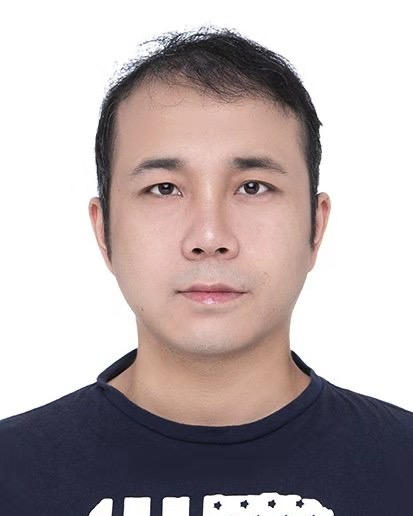
\includegraphics[width=1in,height=1.25in,clip,keepaspectratio]{./photos/Chunfeng_Liu}}] 
{Chunfeng Liu} 
received the bachelor degree in automation from Tsinghua University, Beijing,
China, in 2009 and the master degree in microelectronics from Tsinghua
University, Beijing, China, in 2015. He is currently a PhD student with the Chair
of Electronic Design Automation, Technical University of Munich (TUM). His research interests focus on
computer-aided design for microfluidic biochips. 
\end{IEEEbiography}
\vskip -27.7pt
\begin{IEEEbiography}
[{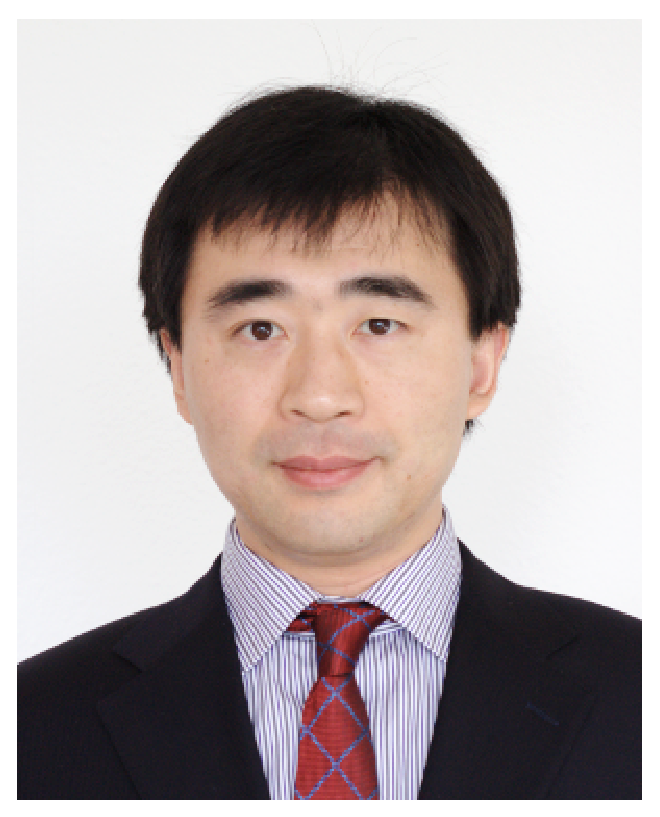
\includegraphics[width=1in,height=1.25in,clip,keepaspectratio]{./photos/Bing_Li}}] 
{Bing Li} 
received the Dr.-Ing. degree from 
Technical University of Munich (TUM), Munich, Germany, in
2010 and finished the Habilitation there in 2018. He
is currently a researcher with the Chair of Electronic
Design Automation, TUM. His current research interests include high-performance and lower-power
design, design automation for microfluidic biochips,
as well as emerging systems. He has served on
the Technical Program Committees of several conferences including ICCAD, DATE,
ASP-DAC, etc.
\end{IEEEbiography}
\vskip -27.7pt
\begin{IEEEbiography}
[{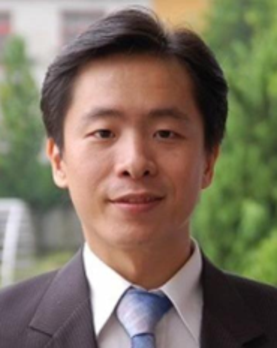
\includegraphics[width=1in,height=1.25in,clip,keepaspectratio]{./photos/Tsungyi}}] 
{Tsung-Yi Ho} (M'08--SM'12) received his Ph.D. degree in Electrical Engineering from National Taiwan
University, Taipei, Taiwan, in 2005.  He is a Professor with the Department of Computer 
Science of National Tsing Hua University, Hsinchu, Taiwan. His research interests include 
design automation and test for microfluidic biochips and nanometer integrated circuits.
Dr. Ho was a recipient of the Best Paper Awards at the VLSI Test Symposium (VTS) in 2013 and IEEE
TCAD in 2015. Currently he serves as an ACM Distinguished Speaker, 
a Distinguished Lecturer of the IEEE Circuits and
Systems Society, and Associate Editor of the ACM JETC, ACM TODAES,
ACM TECS, and IEEE TVLSI, and the Technical Program Committees of
major conferences, including DAC, ICCAD, DATE, ASP-DAC, ISPD, etc.
\end{IEEEbiography}
\vskip -27.7pt
\begin{IEEEbiography}
[{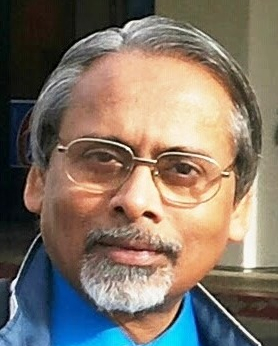
\includegraphics[width=1in,height=1.25in,clip,keepaspectratio]{./photos/BBB_TCAD_Photo}}]
{Bhargab B. Bhattacharya} (F'07) is currently serving as Distinguished Visiting
Professor of Computer Science \& Engineering at the Indian Institute of
Technology Kharagpur. Prior to that, he had been on the faculty of the Indian
Statistical Institute, Kolkata, for over 35 years. His research interest
includes digital logic testing, and electronic design automation for integrated
circuits and microfluidic biochips. He has published more that 400 technical
papers and he holds ten US Patents. He is a Fellow of the Indian National
Academy of Engineering and a Fellow of the National Academy of Sciences
(India).
\end{IEEEbiography}
\vskip -27.7pt
\begin{IEEEbiography}
[{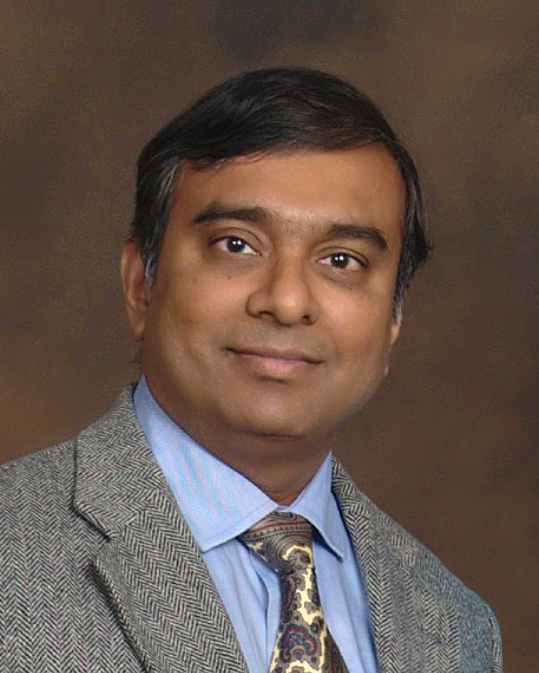
\includegraphics[width=1in,height=1.25in,clip,keepaspectratio]{./photos/Chakrabarty_Krishnendu}}]
{Krishnendu Chakrabarty} (F'08) received the Ph.D. degree from the University of Michigan, Ann Arbor, in 1995. He is now the John Cocke Distinguished Professor and Department Chair of Electrical and Computer Engineering at Duke University. His current research projects include: testing, design-for-testability, and fault diagnosis of 3D SOCs and AI/ML hardware; microfluidic biochips; hardware security. Prof. Chakrabarty is a Fellow of ACM, a Fellow of IEEE, a Fellow of AAAS, and a Golden Core Member of the IEEE Computer Society. 
\end{IEEEbiography}
\vskip -27.7pt
\begin{IEEEbiography}
[{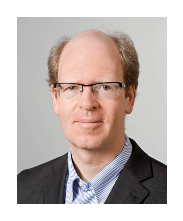
\includegraphics[width=1in,height=1.25in,clip,keepaspectratio]{./photos/Ulf_Schlichtmann}}] 
{Ulf Schlichtmann} (S'88--M'90--SM'18) received the Dipl.-Ing. and Dr.-Ing.
degrees in electrical engineering and information technology from Technical
University  of  Munich (TUM), Munich, Germany, in 1990 and 1995,  respectively.

He is Professor and the Head of the Chair of Electronic Design Automation at
TUM. He joined TUM in 2003, following 10 years in industry. His current
research interests include computer-aided design of electronic circuits and
systems, with an emphasis on designing reliable and robust systems.
Increasingly, he focuses on emerging technologies such as lab-on-chip and
photonics.
\end{IEEEbiography}

\vfill


%\clearpage
%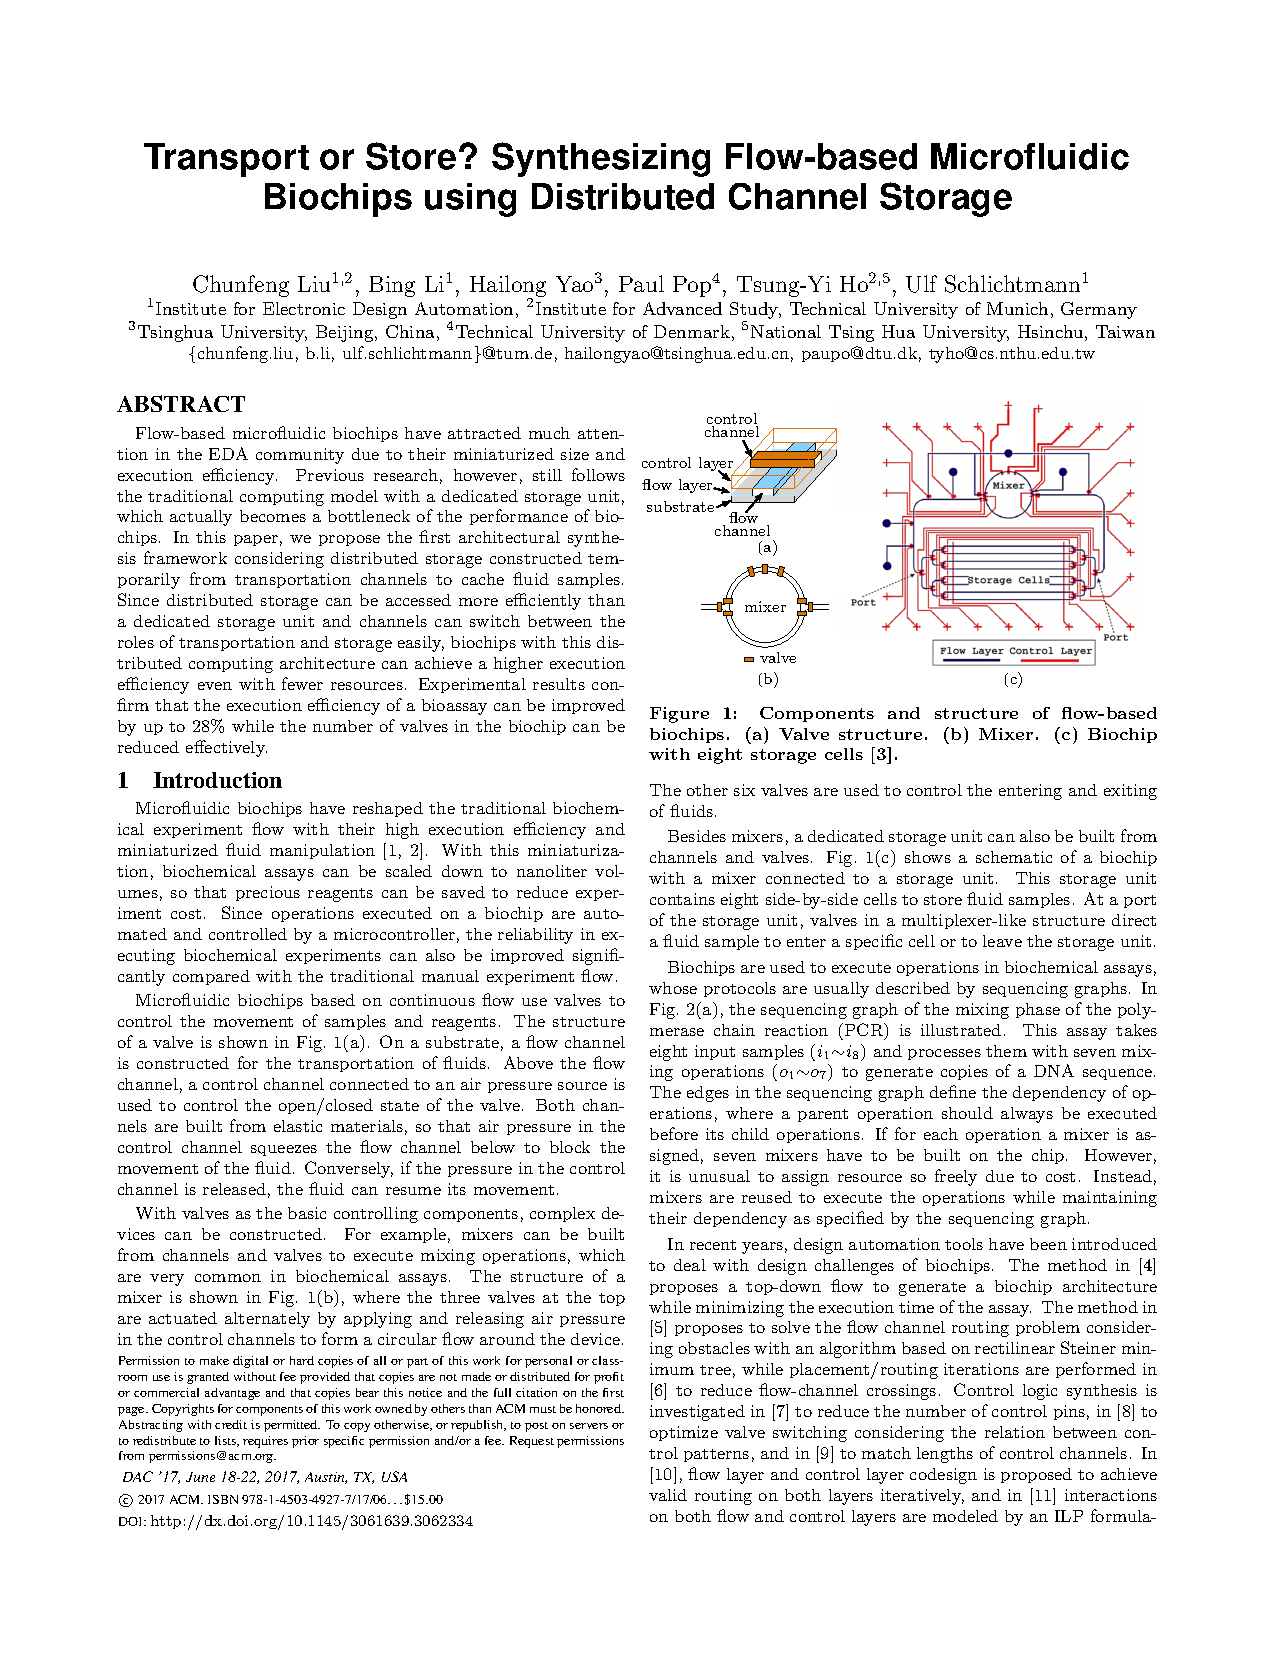
\includepdf[pages=1-last]{a49Liu.pdf}
\end{document}


